\documentclass[english,version-2020-11]{uzl-thesis}
\usepackage{placeins}
\usepackage{microtype}
\usepackage{tikz}
\usepackage{graphicx}
\usepackage{caption} % Package for captions
\usepackage{subcaption} % Package for subfigures

\usetikzlibrary{shapes.geometric, arrows}

\tikzstyle{startstop} = [rectangle, rounded corners, minimum width=3.5cm, minimum height=1cm, text centered, draw=black]
\tikzstyle{process} = [rectangle, minimum width=3.5cm, minimum height=1cm, text centered, draw=black]
\tikzstyle{optional} = [diamond, dashed, minimum width=3cm, minimum height=1cm, text centered, draw=black, aspect=2]
\tikzstyle{data} = [rectangle, minimum width=3.5cm, minimum height=1cm, text centered, draw=black]
\tikzstyle{arrow} = [thick,->,>=stealth]
\tikzstyle{dashedarrow} = [thick, dashed,->,>=stealth]
\tikzstyle{line} = [thick] % Normal line without arrow


%%%

\UzLThesisSetup{
  %
  %
  Logo-Dateiname        = {uzl-thesis-logo-uzl.pdf},
  Verfasst              = {am}{Institut für Software Engineering und Programming Languages},
  %
  % The titles:
  %
  Titel auf Deutsch     = {
    Können semantische Ähnlichkeiten von Wörtern die Schlussfolgerungen des gesunden Menschenverstands verbessern?  Eine Fallstudie mit Prover E und SUMO.
  }, 
  Titel auf Englisch    = {
    Can semantic similarities of words enhance common sense reasoning?  A case study with prover E and SUMO.
  },
  % 
  %
  Autor                 = {Julian Britz},
  Betreuerin            = {Prof. Dr. Diedrich Wolter},
  % 
  % Optional: Supporting persons and institutions. The text should be
  % in German, even for an English thesis.
  %
  Mit Unterstützung von = {Moritz Bayerkuhnlein},
  % 
  %
  Bachelorarbeit,
  Studiengang           = {Informatik},
  %
  % Date on which the thesis is turned in German, formatted the
  % traditional German way:
  %
  Datum                 = {06. Juli 2025},
  %
  % The English abstract. You must always provide abstracts in German
  % and in English. 
  %
  Abstract              = {
    Abstract
  },
  Zusammenfassung       = {
    Zusammenfassung 
  },
  % Bibliography style: Choose between
  % 
    Alphabetische Bibliographie,
  % Alternatively:
  % Numerische Bibliographie
}

\UzLStyle{alegrya modern design}

\addbibresource{thesis_julian_britz-bibtex-entries.bib}

\begin{document}

%
% The title page and table of contents will be inserted automatically
% here. 
%

\chapter{Introduction}
\label{chapter-introduction}

Automated theorem proving is a fundamental technique in formal logic and artificial intelligence. It offers a way to model reasoning tasks in a precise, rule-based framework. A central assumption in this work is that logical reasoning tasks can also capture aspects of natural language understanding. This connection builds on the idea that solving logical problems can serve as a proxy for modeling how meaning and structure in language interact. It enables the validation of logical statements based on a given set of axioms and inference rules. However, the task is computationally difficult in practice. As the search space grows quickly, theorem provers rely on heuristics to guide the proof search. Even then, the success rate remains limited, especially in large or complex domains. Benchmarks like TPTP reflect this challenge and are commonly used to evaluate and compare the performance of provers.

Adimen-SUMO is a first-order logic reengineering of the Suggested Upper Merged Ontology (SUMO), designed to be compatible with automated theorem provers. It formalizes a broad range of commonsense knowledge using logical axioms, allowing provers to reason over structured definitions of entities and their relationships.

Adimen-SUMO’s grammar is closely connected to natural language structures. This means that selecting axioms based on semantic embeddings, which are vector representations of entire sentences capturing their semantic meaning, helps capture underlying logical dependencies that might not be immediately apparent. Frequently used axioms act as structural anchors within this system, making it easier for the theorem prover to navigate the proof search space and discover relevant inference steps. By combining syntactic and semantically relevant axioms with those that have been frequently used in past proofs, the theorem prover benefits from both semantic alignment and structural consistency. This increases the overall proof success rate, as the prover has access to axioms that not only appear relevant but have also proven useful in previous reasoning tasks.

A significant part of this thesis builds upon the work of \cite{Schon2024}, which explores context-specific axiom selection using large language models. Traditional axiom selection methods primarily rely on syntactic properties, often ignoring the meaning embedded in symbol names. Schon proposes an alternative approach by leveraging large language models to determine relevant axioms based on contextual similarity. This method aligns axiom selection with the goal's context, improving performance in commonsense reasoning tasks. Experiments show that this approach outperforms purely syntactic selection methods, demonstrating the potential of semantic similarity for guiding theorem provers.

The following thesis investigates whether incorporating frequently used axioms, referred to as core axioms, into a subset of the Adimen-SUMO ontology improves proof success rates. The selected subset is determined by combining syntactic and semantic criteria to ensure both structural and conceptual relevance.


\section{Problem Statement}
Given a formal logical ontology, such as Adimen-SUMO, and a conjecture \( C \), the objective is to identify a subset of axioms from the ontology that maximizes the probability of proving \( C \). The process involves:
\begin{itemize}
    \item Selecting axioms based on syntactic and semantic similarity, forming a set denoted as \( \mathcal{A}_{\text{rel}} \).
    \item Testing whether adding frequently used axioms, \( \mathcal{A}_{\text{core}} \), improves proof success.
\end{itemize}

Even though there is no direct mapping between natural and logical language, we assume, that there is an entanglement between them. That means both influence each other, and reasoning in one domain can reflect structures in the other. We describe this relation as:\\
\begin{equation}
    \mathcal{L}_{\text{NL}} \bowtie \mathcal{L}_{\text{logic}}
\end{equation}

where \( \mathcal{L}_{\text{NL}} \) stands for the language of natural language expressions, while \( \mathcal{L}_{\text{logic}} \) refers to the formal language used in logical systems like Adimen-SUMO.

Arguments for this assertion are that logical langugage is human made and therefore inevitably connected to human and consequently natural language.
Also ontologies like Adimen-SUMO are partially derived by lexical-semantic networks that capture relationships between words of natural language.
Making use of this entanglement the selection process of theorem proovers can be optimized by reducing the number of relevant axioms.
Theorem prover E follows a refutational proof procedure using the superposition calculus \cite{Schulz2019}. The proof search is based on a modified given-clause algorithm, consisting of several key steps:

\begin{enumerate}
    \item Initialization: The input problem is converted into clausal normal form (CNF) and divided into two sets: unprocessed clauses \( U \) and processed clauses \( P \).
    \item Clause Selection: A clause \( g \) is selected from \( U \) based on heuristics, referred to as the given clause, and is then simplified against \( P \).
    \item Simplification: The given clause undergoes forward simplification using processed clauses. This step removes redundant literals, applies rewriting rules, and ensures that terms are arranged in a canonical order.
    \item Inference: The prover applies the superposition calculus, combining \( g \) with clauses in \( P \) to generate new clauses. These new clauses are simplified and added to \( U \) if they are neither trivial nor redundant.
    \item Saturation or Termination: The process stops when:
    \begin{itemize}
        \item The empty clause \( \bot \) is derived, confirming the proof.
        \item The clause set is saturated, meaning no further inferences can be made.
        \item A predefined resource limit, such as time or memory, is reached.
    \end{itemize}
\end{enumerate}

Axioms play a crucial role in simplification. While the prover cannot arbitrarily discard axioms, as they form the foundation of logical reasoning, they are essential for clause rewriting and subsumption.


\section{Approach}

Before evaluating the effect of frequently used axioms on proof success, the main components of the setup are introduced. The goal is to automatically prove logical properties that have been manually modeled in a formal ontology such as Adimen-SUMO. In this setting, the inclusion of axioms that frequently contribute to successful proofs might support the prover more effectively.

The set of axioms available in Adimen-SUMO is denoted as \( \mathcal{A} \), while \( C \) represents the conjecture to be proven. The similarity between an axiom and the conjecture is measured by a function \( d \).

To refine the axiom selection process, a two-step approach is applied. First, a set \( \mathcal{A}_{\text{rel}} \) is constructed by selecting the \( k \)  axioms, that are most similar to the conjecture according to \( d \):

\begin{equation}
    \mathcal{A}_{\text{rel}} = \{ A \in \mathcal{A} \mid A \text{ is among the } k \text{ closest axioms to } C \text{ w.r.t. } d \}
\end{equation}

In this context, similarity refers to the semantic relatedness between an axiom and the conjecture. This is captured using vector representations of logical expressions. The closeness between axioms is measured using cosine similarity, which quantifies how aligned two vectors are in their direction. A more detailed explanation of this approach follows later in the thesis.
To further filter and prioritize structurally relevant axioms, a syntactic selection strategy is applied to \( \mathcal{A}_{\text{rel}} \). The resulting set, \( \mathcal{A}_{\text{union}} \), forms an optimized selection that maintains both semantic closeness and logical relevance.

Beyond similarity-based and structural selection, a second set \( \mathcal{A}_{\text{core}} \) is constructed from axioms that have been frequently used in past proofs. These axioms act as fundamental inference steps that theorem provers repeatedly rely on.

The final enhanced axiom set \( \mathcal{A}_{\text{enh}} \) is then defined as:

\begin{equation}
    \mathcal{A}_{\text{enh}} = \mathcal{A}_{\text{union}} \cup \mathcal{A}_{\text{core}}
\end{equation}

The function \( P(T, \mathcal{A}', C) \) determins whether a theorem prover \( T \) is able to derive a proof for the conjecture \( C \) using the axiom set \( \mathcal{A}' \). If a proof is found, the function returns true otherwise, it returns false.

\section{Hypothesis}

The hypothesis tested in this thesis is that including frequently used axioms improves the success rate of theorem proving. These axioms are assumed to provide general-purpose inference steps that are useful across many proof tasks. In combination with those selected by syntactic and semantic criteria, they could help the prover resolve gaps that similarity-based methods alone might miss.

Formally, this is expressed as:

\begin{equation}
    \forall C \in \mathcal{C}, \quad \Pr(P(T, \mathcal{A}_{\text{enh}}, C) = \text{True}) > \Pr(P(T, \mathcal{A}_{\text{union}}, C) = \text{True})
\end{equation}

where \( \Pr \) represents the probability of success across a successful proof attempt. This formulation suggests that integrating frequently utilized axioms with those selected through semantic similarity and syntax-based structural relevance enhances the prover’s ability to find a proof more efficiently.


\section{Structure of this Work}

This thesis is structured into several chapters, each addressing different aspects of the research problem and methodology. It begins with an overview of existing research, followed by the theoretical foundations, the proposed approach, experimental evaluations, and concluding discussions.

\textit{Chapter \ref{chapter-relatedwork}} provides a review of related work. It covers previous research on theorem proving and axiom selection techniques, as well as how semantic similarity has been applied in logical reasoning.

\textit{Chapter \ref{chapter-preliminaries}} introduces fundamental concepts necessary to understand the core of this research. It discusses topics such as common sense reasoning, word embeddings, and theorem proving. Additionally, it explains the role of formal grammars and axiom selection in automated reasoning.

\textit{Chapter \ref{chapter-experiments}} focuses on the experimental setup and evaluation. It outlines the benchmark datasets, describes the evaluation metrics, and presents the results of different axiom selection strategies. The impact of incorporating core axioms into theorem proving is analyzed based on empirical findings.

\textit{Chapter \ref{chapter-conclusion}} summarizes the main contributions of this work and highlights key insights gained from the experiments. It also discusses potential future directions and remaining challenges in axiom selection and automated reasoning.

Finally, \textit{Chapter \ref{chapter-futerwork}} explores ideas for future research, suggesting possible extensions and refinements to the proposed approach.

Each chapter builds upon the previous ones, providing a structured progression from theoretical background to practical implementation and evaluation.

% !!!!!!!!!!!!!!!!!!!!!!!!!!!!!!!!!!
% !!! Your action is needed here !!!
% !!!!!!!!!!!!!!!!!!!!!!!!!!!!!!!!!!

\chapter{Related Work}
\label{chapter-relatedwork}
The findings of Schon's work play a crucial role in this thesis, as a major aspect of the proposed approach involves using semantic embeddings for axiom selection.
However, while Schon focuses on direct context-based selection, this thesis investigates the impact of incorporating frequently used axioms into the selection process. The goal is to determine whether combining core axioms with those chosen based on semantic similarity enhances proof success rates.

Beyond Schon's work, several other studies have contributed to axiom selection and theorem proving. Adimen-SUMO, developed by Alvez et al. \cite{Alvez2014}, is a reengineered version of the SUMO ontology designed to improve compatibility with first-order theorem provers. The restructuring ensures that axioms are formulated in a way that facilitates inference, reducing ambiguities present in the original SUMO. This ontology serves as a key resource in evaluating theorem provers, including those used in this thesis.

Syntactic axiom selection has also been widely explored. \cite{Hoder2011} introduced SInE, a system that selects axioms based on their syntactic relevance to the conjecture. By iteratively choosing axioms that introduce symbols appearing in the conjecture, SInE reduces the search space, making large knowledge bases more manageable.

Another relevant contribution comes from \cite{Alvez2017}, who introduced a framework for systematic WhiteBox testing of first-order logic ontologies. Their work focuses on ensuring logical consistency and eliminating redundant or contradictory axioms. Automated testing techniques from this study provide insights into ontology refinement, which is relevant when evaluating the quality of selected axioms in theorem proving.

In summary, Schon's research serves as the primary foundation for this thesis, providing a framework for semantic axiom selection that is further extended through the integration of frequently used axioms. Other related studies on syntactic axiom selection, ontology structuring, and logical consistency contribute valuable insights, supporting the refinement of the proposed approach.

% !!!!!!!!!!!!!!!!!!!!!!!!!!!!!!!!!!
% !!! Your action is needed here !!!
% !!!!!!!!!!!!!!!!!!!!!!!!!!!!!!!!!!

\chapter{Preliminaries}
\label{chapter-preliminaries}

This chapter introduces fundamental concepts relevant to this work. It covers common sense reasoning, word embeddings, formal grammars, automated theorem proving, and axiom selection strategies. These topics form the theoretical foundation for the experiments and analyses presented in later chapters.

\section{Common Sense Reasoning}

Common sense reasoning is an essential part of human cognition, allowing individuals to understand everyday situations, infer unstated knowledge, and make reasonable decisions even when information is incomplete. Automated reasoning systems attempt to replicate this ability to improve inference and decision-making.

Common sense reasoning involves recognizing unstated premises in logical arguments, understanding cause-effect relationships, and applying heuristics to solve problems under uncertainty. It plays a key role in artificial intelligence, particularly in natural language understanding, where context is crucial for interpreting meaning, and in automated reasoning, where structured logical frameworks help infer conclusions from available premises. Modern applications further highlight the importance of integrating knowledge-based reasoning for interpretability and reliability. Despite advancements in AI, these models struggle with incorporating structured and generalizable knowledge, making common sense reasoning an ongoing challenge.

Interpreting a sentence often involves more than just processing its words, it requires incorporating background knowledge to make sense of implicit information. Take, for example, the Winograd Schema involving John and Billy viewing a stage \cite{Levesque2012}. 
"John could'nt see the stage with Billy in front of him because he is so short."
While the sentence itself is simple, understanding it correctly depends on a series of assumptions that humans naturally make when constructing a mental model of the situation \cite{Bayerkuhnlein2023}.

A stage is something meant to be viewed. In a typical setting, viewers remain stationary, and obstructions can block their line of sight. Humans are physical entities, meaning they cannot see through solid objects. Both John and Billy are human names, so the sentence suggests a scene where one person is obstructing the other’s view. The interpretation of who is blocking whom depends on the additional context provided by the sentence, but the reasoning process remains the same: we piece together knowledge about how the world works to arrive at a coherent understanding.

These intuitive assumptions form the foundation of common sense reasoning. The process aligns with the theory of mental models, which suggests that humans construct internal representations of a scenario to evaluate possible interpretations \cite{JohnsonLaird1989}. In the case of ambiguous pronouns, this internal model helps determine which assignment makes the most logical sense. This ability to build structured mental representations is what allows humans to effortlessly resolve ambiguities that challenge AI systems.

\section{Grammars in Natural and Formal Languages}

Understanding language through logic-based approaches often involves representing meaning in a structured and interpretable way. In this context, grammars and lexicons provide the foundation for mapping natural language expressions into formal representations. A lexicon connects linguistic elements, such as words or phrases, to their logical counterparts, while grammars define how these elements can be combined to form valid expressions. This interplay between lexicon and grammar is central to logic-based natural language understanding (NLU), where the goal is to derive logical forms from language that can be used for reasoning.

Grammars define the structural rules of a language, whether it is a natural language like English or a formal system used in logic. In theorem proving, grammars are essential for structuring logical statements in a way that machines can interpret and manipulate.

Different types of grammars serve various purposes. Context-free grammars (CFGs) define syntactic structures in natural language processing and programming languages. First-order logic (FOL) grammars represent logical expressions using predicates, functions, and quantifiers. Ontology-based grammars, such as SUMO (Suggested Upper Merged Ontology), combine linguistic and logical structures to improve knowledge representation \cite{Niles2001}.

Grammars are crucial in theorem proving because they enforce logical consistency, allow automated systems to process logical expressions systematically, and provide a structured representation of knowledge in formal systems like SUMO and Adimen-SUMO. Adimen-SUMO is written in Thousands of Problems for Theorem Provers (TPTP) Syntax, a standardized language designed for expressing logical problems in automated reasoning \cite{Alvez2014}. TPTP, originally developed to facilitate the benchmarking and comparison of theorem provers, provides a well-defined structure for first-order logic expressions, ensuring compatibility across different proving systems. By using TPTP, Adimen-SUMO maintains a formal and machine-readable representation of axioms, allowing theorem provers to efficiently process and reason over its logical content.

In TPTP syntax, axioms are typically expressed in First-Order Form (FOF), which represents first-order logic statements in a structured and readable format. The FOF format explicitly defines logical components such as axioms, conjectures, and definitions, ensuring clarity in automated reasoning tasks. An example of an axiom in Adimen-SUMO written in FOF syntax is:


\begin{Pseudocode}[morekeywords = {add, create}, deletekeywords={to}, numbers=left,
    caption = {Axiom example Adimen-SUMO}]
    fof(predefinitionsA7, axiom,
        (![X]: 
            (
                p__d__subclass(X, X)
            )
        )
    ).
\end{Pseudocode}

This axiom states that for all entities \( X \), \( X \) is always a subclass of itself. In natural language, this expresses the reflexive property of the subclass relation, meaning that every class is considered a subclass of itself. This kind of axiom is fundamental in ontology-based reasoning, as it helps maintain consistency within hierarchical structures.

\section{Word Embeddings and Semantic Similarity}

Word embeddings represent words as numerical vectors in a continuous space, capturing semantic relationships based on their contextual usage. Unlike traditional representations such as one-hot encoding, embeddings enable words with similar meanings to be positioned closer together in the vector space. This makes it possible for models to generalize across linguistic variations and draw inferences from meaning-based relationships.
Words are considered semantically similar when they appear in similar contexts. However, closeness in the embedding space does not imply pure synonymy, rather, it reflects a broader notion of relatedness grounded in context. This means that embeddings capture not only similarity but also functional and associative relationships between words, since words used in similar contexts often share some underlying conceptual or syntactic role.

One of the well-known demonstrations of this structure is the analogy example: the vector operation \textit{man - woman + queen} results in a vector that is close to \textit{king}. This shows that embeddings can model more than just pairwise similarity—they encode directional relationships that reflect conceptual patterns, allowing analogical reasoning over word vectors. These kinds of regularities are what make embeddings so powerful for downstream tasks like axiom selection, where relational structure matters. \cite{Mikolov2013}

\begin{figure}[h!]
    \centering
    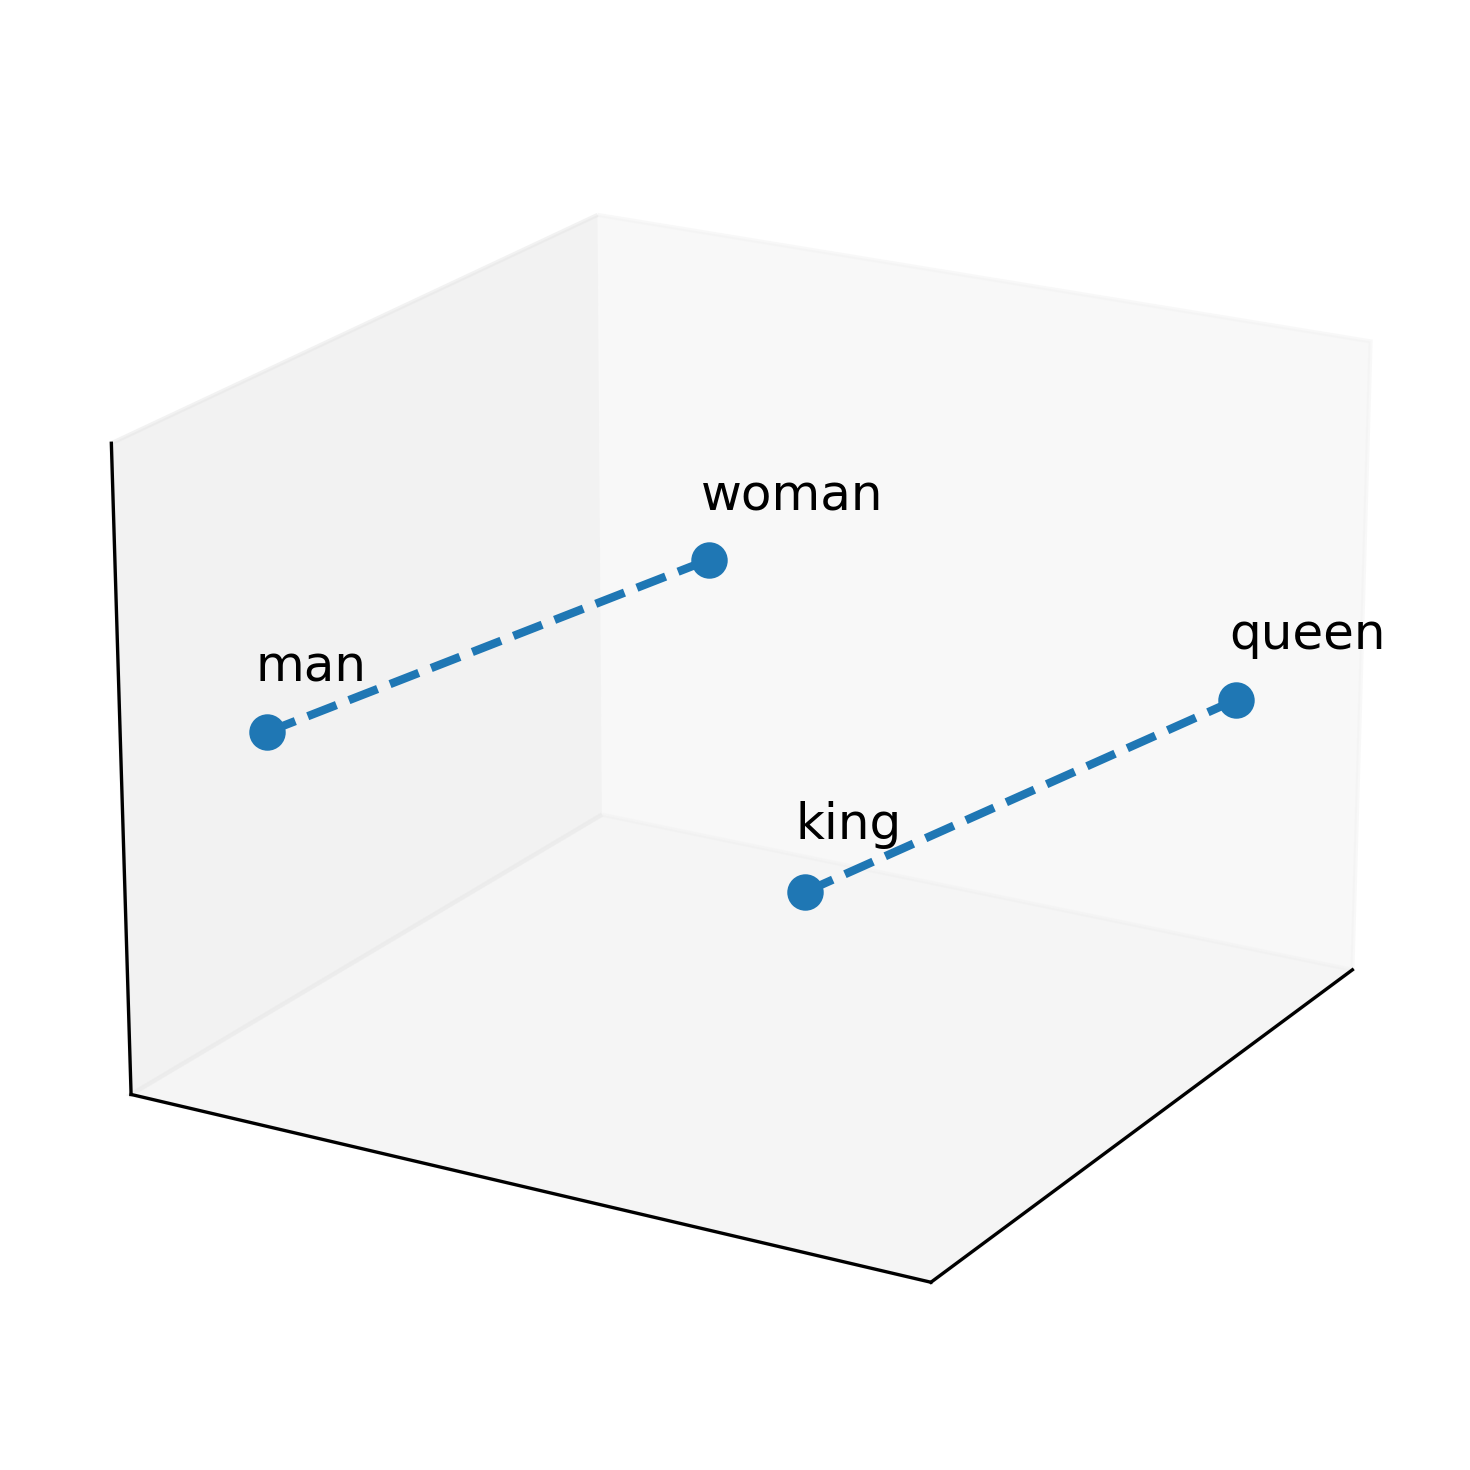
\includegraphics[width=\textwidth]{embedding_analogy.png}
    \caption{Embedding analogy}
    \label{fig:embedding_analogy}
\end{figure}
\FloatBarrier

Different techniques have been developed to generate word embeddings, each with unique properties and advantages. Word2Vec \cite{Mikolov2013} is one of the foundational models, introducing two architectures: Continuous Bag of Words (CBOW) and Skip-gram. CBOW predicts a word based on its surrounding context, while Skip-gram does the inverse, predicting context words given a target word. This approach efficiently captures both syntactic and semantic relationships. FastText \cite{Bojanowski2017} extends Word2Vec by incorporating subword information, representing words as bags of character n-grams. This allows it to handle rare words and out-of-vocabulary terms better than standard word-based models. GloVe \cite{Pennington2014}, in contrast, constructs embeddings by factorizing a word co-occurrence matrix, capturing both local and global semantic information.

\begin{figure}[h]
    \centering
    \begin{subcaptionblock}{0.45\textwidth}
        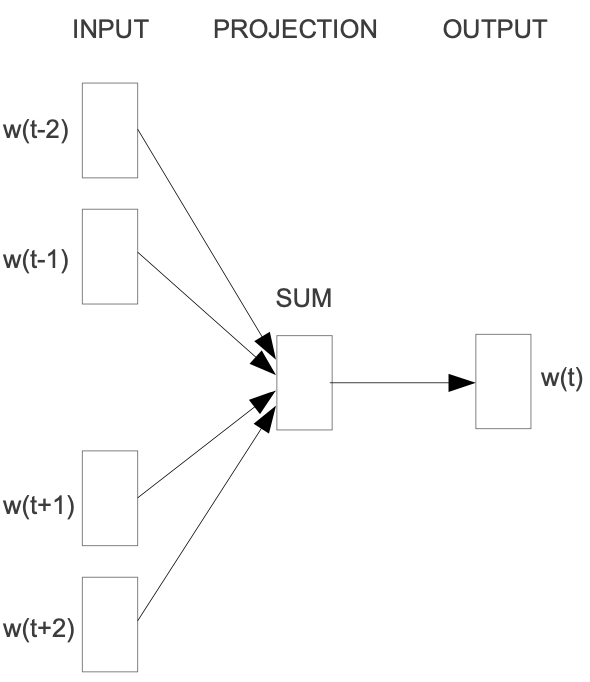
\includegraphics[width=\linewidth]{cbow.png}
        \caption{CBOW Model}
    \end{subcaptionblock}
    \hfill
    \begin{subcaptionblock}{0.45\textwidth}
        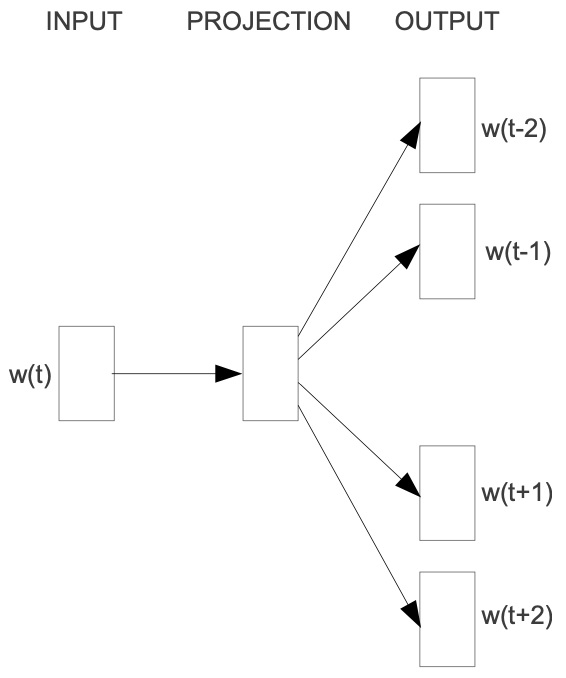
\includegraphics[width=\linewidth]{skip_gram.png}
        \caption{Skip-Gram Model}
    \end{subcaptionblock}
    \caption{Comparison of CBOW and Skip-Gram Models}
\end{figure}


The effectiveness of word embeddings depends on several factors, including the size of the context window, the type of training data, and the inclusion of subword information.

Beyond standard word embeddings, contextual embeddings such as BERT and GPT further refine representation by considering the full sentence structure, allowing word meanings to dynamically change based on context \cite{Devlin2019}. This advancement is particularly relevant in cases where words have multiple meanings depending on their use in different sentences.

In this work, word embeddings are leveraged to determine the semantic similarity between axioms and conjectures. By using pre-trained models like SBERT, it becomes possible to enhance axiom selection in theorem proving, ensuring that the selected axioms are not only structurally relevant but also semantically meaningful.

\section{Automated Theorem Proving}

Automated theorem proving aims to determine whether a given conjecture follows logically from a set of axioms. It is a key component of formal logic and artificial intelligence.

Theorem provers rely on different proof strategies. Logical inference derives new statements from existing ones using formal rules. Resolution is a proof technique that derives contradictions, commonly used in first-order logic provers. Refutation works by attempting to show that a conjecture holds by deriving a contradiction from its negation.

Prover E is a widely used theorem prover based on the superposition calculus \cite{Schulz2019}. Another prominent theorem prover is Vampire \cite{Riazanov2002}.

\section{Axiom Selection Strategies}

First-order logic is undecidable in general, meaning that there exists no algorithm that can determine the provability of every possible statement within finite time. However, automated theorem provers attempt to approximate this task using heuristics and efficient search strategies. When applied to large or complex knowledge bases, the size of the search space quickly becomes intractable, often making exhaustive proof attempts computationally infeasible.

This makes axiom selection a critical component of the proving process. By reducing the number of axioms considered during proof search, the prover is guided more efficiently toward relevant inference steps, improving both performance and the overall proof success rate.


\section{Syntax-Based Selection: SInE}

The SInE selection strategy is a trigger-based approach designed to efficiently select axioms in automated theorem proving \cite{Hoder2011}. Instead of selecting axioms based on fixed rules, it dynamically determines relevance using a trigger relation. This relation ensures that an axiom is only selected if at least one of its symbols appears less frequently than or as frequently as all other symbols in the axiom. This prevents highly common symbols from triggering every axiom they appear in, reducing unnecessary selections.

The selection process starts by identifying symbols that appear in the conjecture to be proven. These symbols are considered directly triggered. If a triggered symbol appears in an axiom and satisfies the trigger relation, the axiom is selected, and its other symbols become triggered in the next selection step. This process continues recursively up to a defined depth \( k \), ensuring that only the most relevant axioms are included.

One limitation of this approach arises when an axiom contains symbols with nearly equal occurrence counts. In such cases, only the least frequent symbol can trigger the axiom, potentially excluding useful axioms. To address this, a benevolence parameter \( b \) is introduced, allowing symbols that occur up to \( b \) times more frequently than the least common symbol to also act as triggers. This adjustment provides more flexibility in axiom selection.

\section{Vector-Based Selection}

Syntax-based selection methods like SInE do not consider the meaning of symbol names, which can lead to the loss of useful information. This is particularly problematic in commonsense reasoning, where symbol names often carry semantic meaning that could improve selection. To address this, vector-based selection methods leverage word embeddings to quantify the semantic similarity between axioms and the goal.

As seen above, word embeddings are a common technique in natural language processing, based on the distributional hypothesis \cite{Miller1991}. This hypothesis states that words appearing in similar contexts tend to have similar meanings. By training neural networks on large text corpora, words are mapped into a continuous vector space, where their geometric positions capture semantic relationships. Cosine similarity is commonly used to measure the closeness of two word vectors, with values ranging from -1 (completely dissimilar) to 1 (identical).

ANMERKUNG VON PROF. DR. WOLTER UNKLAR BEZÜGLICH \( \mathbb{u}^t \)  
-> tbd  

\begin{definition}
    Let \( u, v \in \mathbb{R}^n \) be non-zero vectors. The cosine similarity of \( u \) and \( v \) is defined as:
    \begin{equation}
        \operatorname{cosine\ similarity}(u, v) = \frac{u \cdot v}{\|u\| \cdot \|v\|}
    \end{equation}
\end{definition}

Schon \cite{Schon2023} introduces a statistical approach for axiom selection that relies on word embeddings to represent axioms as vectors. The idea is to encode axioms into a continuous vector space where axioms that occur in similar contexts — and thus share semantic or structural relationships — are mapped closer together. This is done in a preprocessing step, where each axiom in the knowledge base is transformed into a vector representation using a word embedding model.

When selecting axioms for a given conjecture \( C \), the goal is vectorized in the same way as the axioms in the knowledge base. The selection process then identifies the \( k \) axioms whose vector representations are most similar to that of \( C \). The similarity between vectors is measured using cosine similarity, which quantifies how closely two vectors align regardless of their magnitude.

Formally, given a knowledge base \( KB \), a conjecture \( C \), and a vectorization function \( f \) that maps axioms to \( \mathbb{R}^n \), the vector-based selection process selects the \( k \) axioms in \( KB \) that have the highest cosine similarity to \( C \). The selected axioms form a subset of \( KB \) where no other axiom outside this subset has a higher similarity to \( C \) than the least similar axiom within the selected set.

This approach is based on the assumption that prioritizing axioms with high semantic similarity to the goal should lead to more relevant selections and, in turn, increase the likelihood of finding a successful proof.

ANMERKUNG ZUM KOMMETAR VON PROF. DR. WOLTER:  
Die Abgrenzung liegt darin, dass dieser Abschnitt vorstellt, dass man auch ganze Sätze in den Vektorraum einbetten kann, um somit ganze Axiome einbetten zu können. Der Abschnitt baut thematisch natürlich auf dem Kapitel Word Embedding auf - fügt sich m.E. allerdings hier in die Reihe nach Sytax-Based Selection und Vector-Based Selection gut ein, da dies auch dem Step-by-Step vorgehen in der Arbeit von Claudia Schon entspricht. Zudem liefert der Abschnitt den Übergang zur sehr wichtigen Beschreibung des Vorgehens bei der Kombination aus SInE und SeVEn.  
-> tbd  

\section{SeVEn: Sentence-Based Vector Encoding}

Sentence embeddings function similarly to word embeddings, as they are also generated by training neural networks on large text corpora. However, while word embeddings focus on individual words, sentence embeddings capture the meaning of entire sentences or even full documents \cite{Kiros2015SkipThought}. This ability makes them particularly useful for encoding more complex relationships between axioms.

Following this idea, the SeVEn approach builds upon vector-based selection by modifying how axioms are represented. Instead of encoding individual symbol names, each axiom is first translated into a sentence that captures its semantic meaning. This sentence is then encoded into a vector using a sentence embedding model. The overall process remains similar to standard vector-based selection, but the vectorization method is adapted to work at the sentence level. Given a knowledge base \( KB \), where each axiom \( A \) is transformed into a sentence \( S \) using a function \( t \), the sentence embedding function \( f \) then maps \( S \) into a vector representation \( v_S(A) \). The full sentence-based vector representation of the knowledge base is denoted as \( v_S(KB) \), where each axiom is now represented as a sentence embedding.

This adaptation allows SeVEn to leverage the richer semantic information captured in sentence embeddings while maintaining the core structure of vector-based selection.

\section{Combining Vector-Based and Syntactic Selection}.

Building on this idea, \cite{Schon2023} introduced a hybrid approach that integrates SeVEn with the syntactic selection method of SInE. The process starts by expanding the goal with axioms selected through SeVEn. Then, SInE is applied to this extended set of conjectures, selecting additional axioms based on its trigger-based mechanism. 

Using formal notation, let \( \text{sine}(KB, \{A_1, ..., A_n\}) \) represent the axioms selected by SInE for a set of conjectures, and let \( \text{seven}(KB, C) \) denote the axioms selected by SeVEn for a conjecture \( C \). The combined selection strategy is then defined as:

\begin{definition}
    \begin{equation}
        \text{union}(KB, C) = \text{sine}(KB, C \cup \text{seven}(KB, C))
    \end{equation}
\end{definition}

This formulation allows for flexibility in axiom selection, as different selection strategies can be incorporated depending on the specific needs of the reasoning task.

% !!!!!!!!!!!!!!!!!!!!!!!!!!!!!!!!!!
% !!! Your action is needed here !!!
% !!!!!!!!!!!!!!!!!!!!!!!!!!!!!!!!!!

\chapter{Experiments}
\label{chapter-experiments}

This chapter presents the experimental setup and evaluation of different axiom selection strategies in the context of automated theorem proving. The work is situated at the intersection of semantic similarity-based selection and structural optimization of axiom sets, aiming to improve proof success rates in large ontologies like Adimen-SUMO.

The experiments address two main objectives. First, they reengineer and validate the results of Claudia Schon's work \cite{Schon2024}, which proposed a semantic selection method using sentence embeddings for commonsense reasoning. This serves as a baseline and ensures the reproducibility and correctness of prior claims. Second, the experiments test the central hypothesis of this thesis: that proof success improves when axioms frequently used in past proofs—referred to as core axioms—are systematically added to a set of semantically and syntactically relevant axioms.

The evaluation is structured as follows: WhiteBox tests are used to assess logical consistency and inference capabilities; different selection strategies are compared in terms of proof coverage and time performance; and multiple theorem provers are tested to examine the generalizability of the approach. Together, these experiments aim to verify the stated hypothesis and provide a broader classification of the strengths and limitations of current axiom selection techniques.


\section{Construction of WhiteBox Tests}

The methodology for constructing WhiteBox tests follows the approach described by Alvez \cite{Alvez2017}. The tests are designed to assess the logical consistency and inference capabilities of theorem provers by introducing controlled variations in axiom selection.

In the context of Adimen-SUMO, truth tests are constructed as logical conjectures that should be provable based on the ontology's axioms. These tests are essential for evaluating the consistency and reasoning capabilities of automated theorem provers. By verifying that the expected logical consequences can be derived, truth tests help assess the completeness and correctness of the knowledge representation. 

An example of a WhiteBoxTruth test in Adimen-SUMO is the following:

\begin{Pseudocode}[morekeywords = {add, create}, deletekeywords={to}, numbers=left,
    caption = {WhiteboxTruthTest example}]
    fof( whiteBoxTruthTest2824, conjecture,
        (?[MORPH]: 
            (
                ~ (
                    p__d__instance(MORPH,c__Morpheme)
                )
            )
        )
    ).
\end{Pseudocode}


The expression states that there exists at least one entity, represented by the variable \( MORPH \), for which the predicate \( p\_\_d\_\_instance(MORPH, c\_\_Morpheme) \) does not hold. In simpler terms, it asserts that at least one entity is not an instance of the class "Morpheme."

By negating the statement that all instances belong to the class "Morpheme," this test challenges the theorem prover to derive a contradiction if the ontology implies that every entity must belong to this class. If a contradiction is found, it confirms that the original classification of "Morpheme" is inconsistent, helping to assess the reasoning capabilities of the prover.

\section{Reengineering of Prior Work}

To evaluate different axiom selection techniques, this work reengineers the results presented in \cite{Schon2024}. The primary goal is to validate previous findings while assessing the impact of alternative selection methods. The evaluation compares three selection approaches: syntactic selection using SInE, semantic selection based on SeVEn, and a hybrid \textit{union} approach combining both methods.

Each method is tested under the same conditions using a randomly selected subset of 1,000 WhiteBoxTruth tests from Adimen-SUMO. Theorem prover E is used with a fixed configuration, ensuring consistent input formatting and a time limit of 15 seconds per proof attempt:

\begin{Pseudocode}[morekeywords = {add, create}, deletekeywords={to}, numbers=left,
    caption = {Command to run Prover E}]
    eprover --tstp-format --soft-cpu-limit=15
\end{Pseudocode}

For syntactic selection, the SInE strategy is applied with a benevolence parameter of 3 and a recursion depth of 2. In contrast to prior work, the number of selected axioms in the semantic analysis is increased to 1,500, which is three times higher than the previous maximum. This adjustment is made to align the number of selected axioms with the average output of the SInE strategy, ensuring comparability between the syntactic and semantic runs.

The hybrid approach, which combines vector-based SeVEn and syntactic selection, is configured as follows:

\begin{itemize}
    \item The sentence embedding model used is the pre-trained all-MiniLM-L6-v2 from SentenceTransformer, featuring 384 dimensions and a model size of 80MB. It was trained by Reimers et al. on a large dataset of over 1 billion training pairs and is optimized for diverse NLP tasks \cite{Reimers2019, Sentencetransformers2019}.
    \item The number of closest axioms \( k \) selected for each conjecture \( C \) is set to 160.
    \item The SInE parameters remain the same as in the syntactic selection: benevolence = 3, recursion depth = 2.
\end{itemize}

Since the \textit{union} approach applies the SInE strategy to a broader set of initial axioms than the purely syntactic selection, the final number of selected axioms is also higher, averaging around 1,800. This increase reflects the integration of both semantic and syntactic relevance in axiom selection, aiming to enhance the theorem prover’s ability to find proofs efficiently.

The prover results are categorized into:
\begin{itemize}
    \item \textit{Timeout:} Instances where the automated prover exceeded the allocated computational resources without deriving a proof.
    \item \textit{Proof Found:} Instances where the prover successfully established a proof within the given constraints.
    \item \textit{Gave Up:} Instances where the prover terminated prematurely without reaching a conclusive result.
\end{itemize}

\begin{figure}[ht]
    \centering
    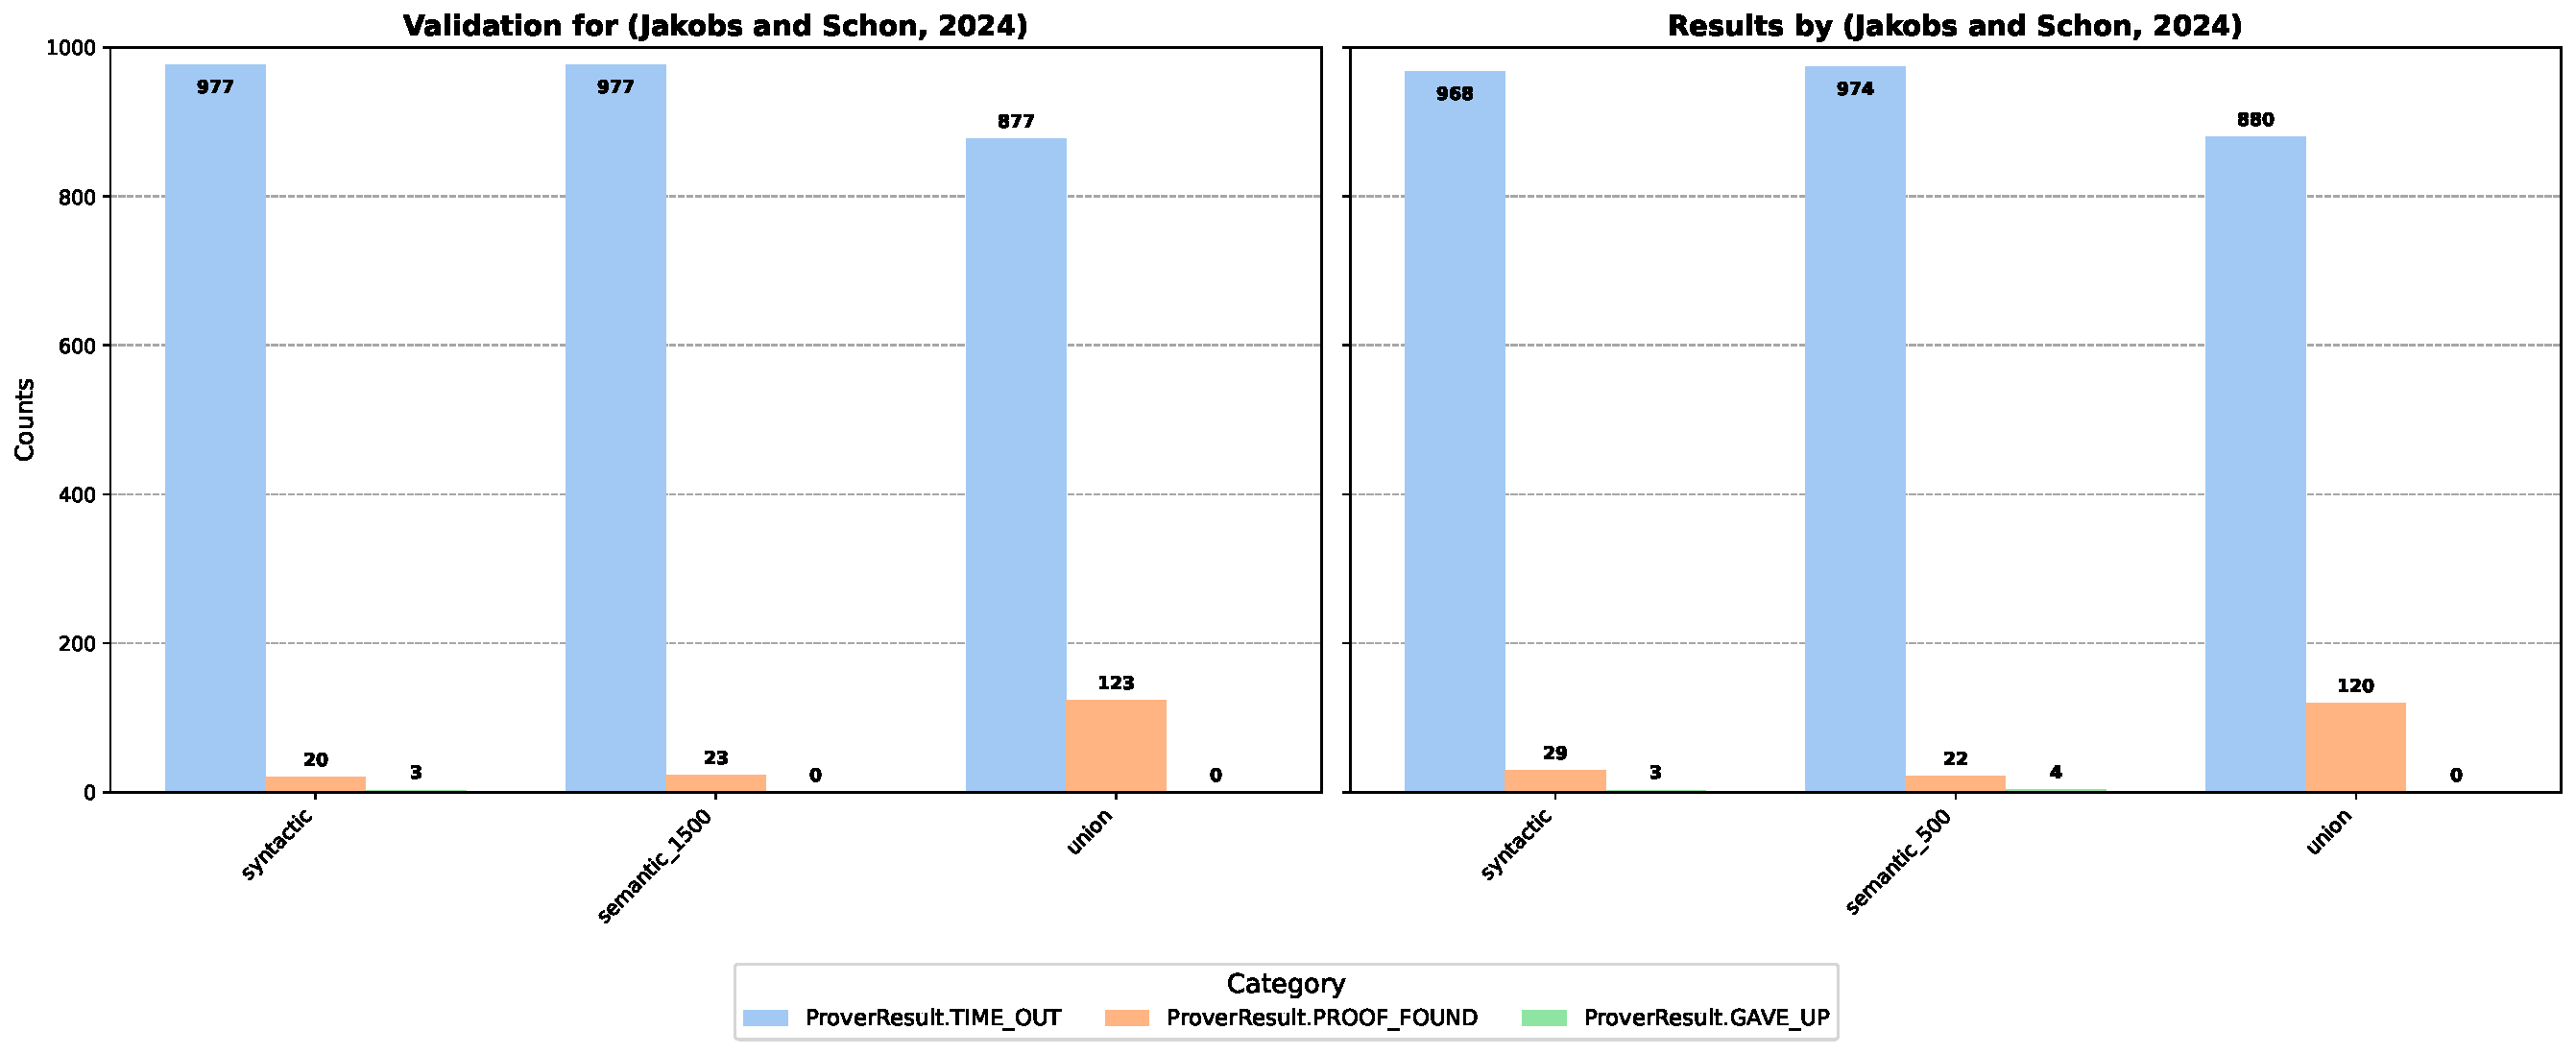
\includegraphics[width=\textwidth]{comparison_output.pdf}
    \caption{Validation for and results of \cite{Schon2024}}
    \label{fig:reengineering}
\end{figure}

\subsection{Interpretation of the Results}

The results in \ref{fig:reengineering} correspond to the prior investigations. While a purely syntactic and purely semantic approach can only find few proofs in the given time, the combination can achieve better results.
These results support the validity of the semantic selection method proposed by \cite{Schon2024}, confirming that the approach can be reproduced and leads to comparable outcomes.
Nevertheless, a significant portion of test cases resulted in timeouts or failed proof attempts. But also for the combination the overall success rate remained low.
The findings suggest that relying solely on semantic similarity in combination with a syntactical selection precedure is not sufficient for effective axiom selection. Future experiments should investigate whether incorporating frequently used core axioms can enhance proof success rates. Additionally, exploring the relationship between axiom complexity and proof outcomes may offer deeper insights into theorem proving behavior, ultimately leading to more refined selection strategies.


\section{Analysis of Reengineering}

To get an indication and possibly recognize patterns for which conjectures the prover could find proofs, the results of the previous \textit{union} run are examined. To understand the factors affecting the success of proof search in theorem proving, several characteristics of the conjectures are examined. Specifically, the influence of the number of variables, the presence of logical operators, and the overall character count in a conjecture are analyzed. These elements contribute to the complexity of the search space and potentially impact the likelihood of finding a proof.

Since each variable expands the number of possible substitutions and inferences the prover must consider, a higher number of variables generally results in a larger search space. It is expected that conjectures with fewer variables are easier to prove, as the prover has to evaluate fewer possible cases.

First-order logic relies on specific symbols as logical operators, each contributing to the structural complexity of a conjecture. The most relevant symbols and there frequency over all 1.000 WhiteboxTruthTests include:
\begin{itemize}
    \item \texttt{|} (disjunction) : 341
    \item \texttt{\&} (conjunction) : 1.224
    \item \texttt{?} (variable indicator) : 1.029
    \item \texttt{!} (universal quantifier) : 90
    \item \texttt{\~{}} (negation) : 798
\end{itemize}

These numbers show that conjunctions and variable indicators occur most frequently, indicating that many conjectures consist of multiple connected clauses and variable bindings. Negations also appear prominently, which suggests that many statements are formulated as refutations or logical contradictions—typical in automated reasoning setups. Disjunctions and universal quantifiers are less common in comparison.


A higher occurrence of these symbols increases the structural complexity of a conjecturecit \cite{Dantsin2001}. More complex logical expressions require additional inference steps, making it more challenging for the theorem prover to find a proof. Therefore, it is expected that conjectures with fewer logical operators are more likely to be proven within a limited time.

Lastly, the overall character count of a conjecture is analyzed as a general measure of complexity. Longer conjectures tend to introduce more structural elements, increasing the reasoning effort required by the prover. By examining how the length of a conjecture correlates with proof success rates, it is possible to determine whether shorter conjectures are indeed easier to prove.

The following presents the results of these analyses, comparing proof success rates based on these complexity factors. The implications of these findings are then discussed in detail, highlighting how different structural properties influence theorem proving performance.


\begin{figure}[h!]
    \centering
    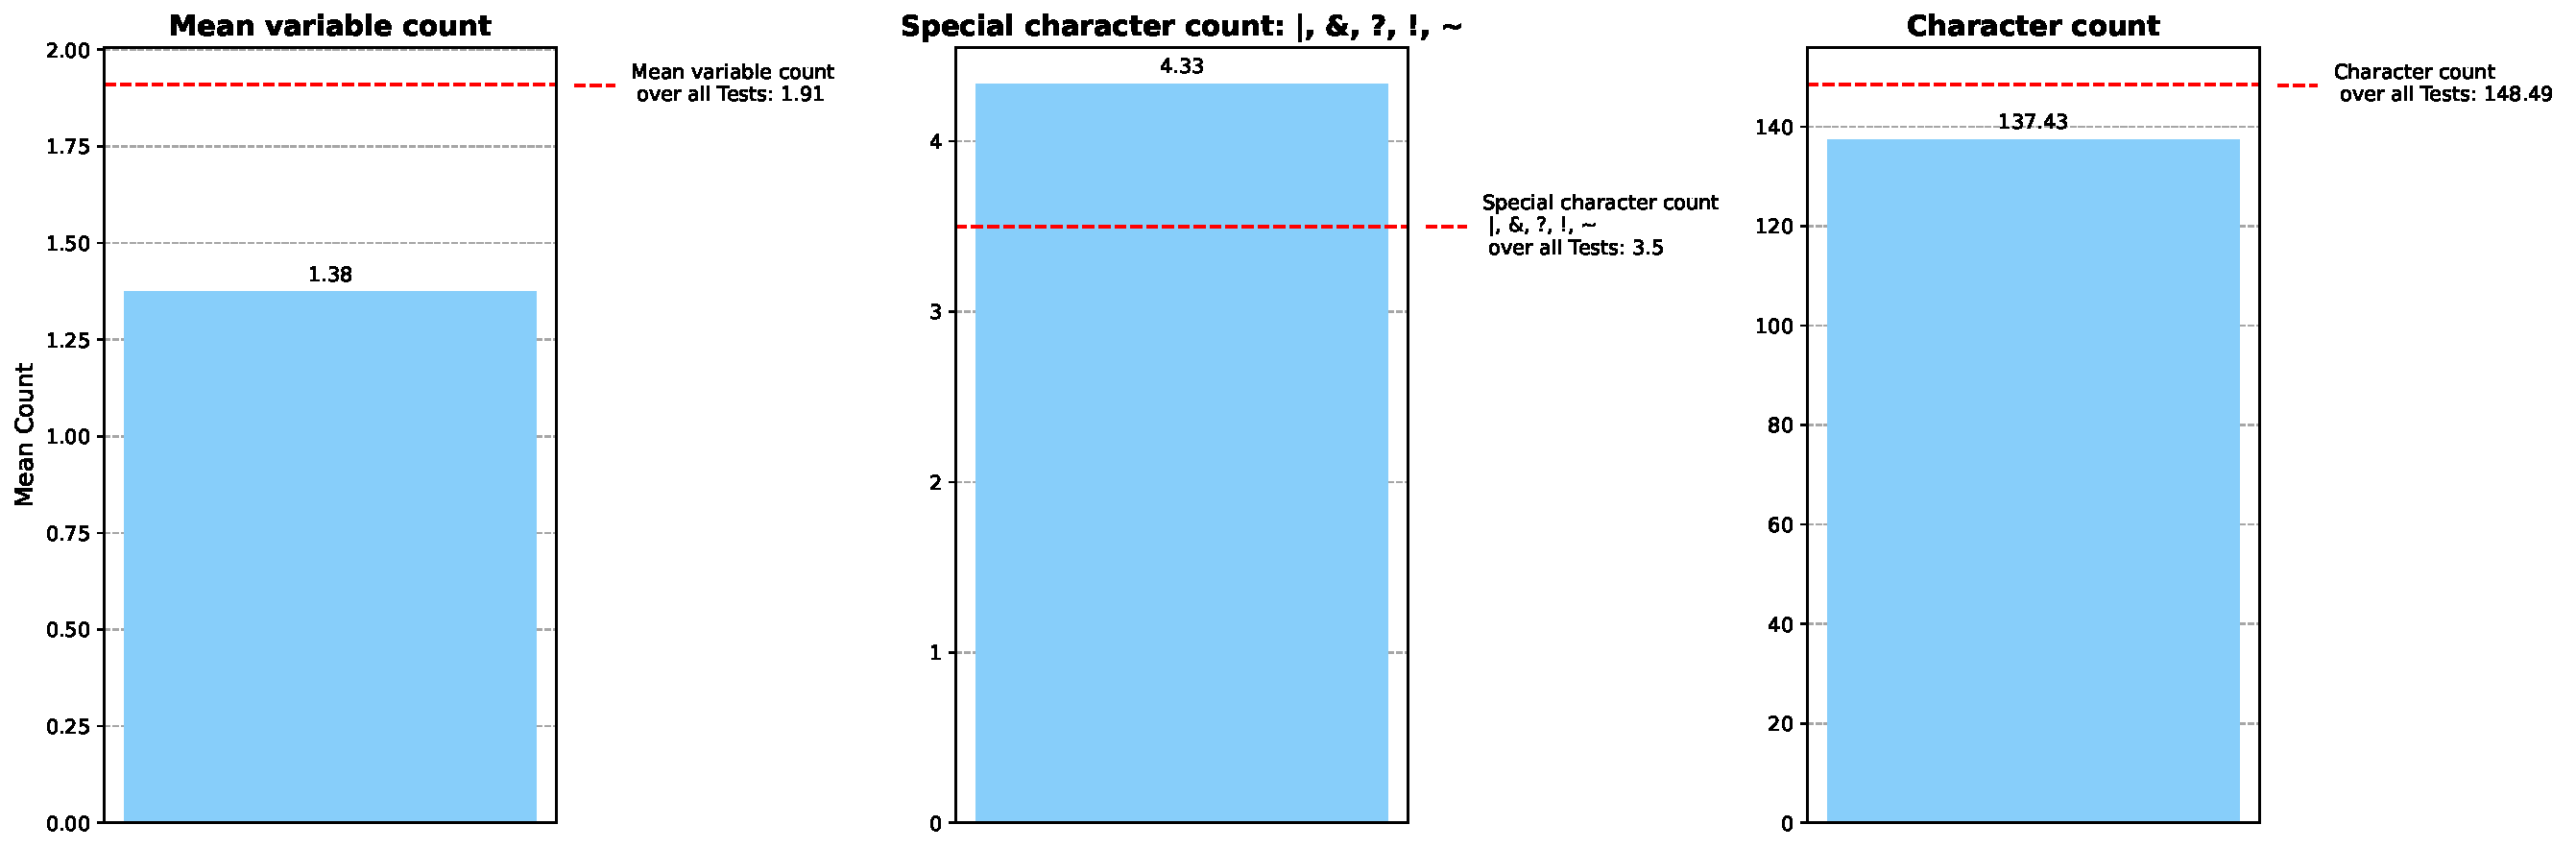
\includegraphics[width=\textwidth]{combined_graphs.pdf}
    \caption{Analysis of Reengineering}
    \label{fig:analysis_reeingieering}
\end{figure}
\FloatBarrier

The average number of variables in conjectures where proofs are found is 1.38, clearly below the overall average of 1.91. Similarly, the count of special characters such as \texttt{|}, \texttt{\&}, \texttt{?}, \texttt{!}, and \texttt{\textasciitilde} stands at 4.33, compared to the overall mean of 3.5. The average character count in successful proofs is 137.43, slightly lower than the global average of 148.49.
The results confirm that all examined factors influence the success rate of theorem proving as expected. Conjectures with fewer variables consistently yielded higher proof success rates, supporting the assumption that an increase in the number of variables expands the search space, making proof discovery more challenging.

Similarly, the impact of logical operators aligns with expectations. Conjectures containing a higher number of disjunctions, conjunctions, quantifiers, and negations were significantly harder to prove.

The general character count of a conjecture also showed a correlation with proof success. Conjectures with a lower character count were proven more frequently, reinforcing the idea that shorter conjectures introduce fewer structural elements that could complicate reasoning. While character count alone is not a direct measure of complexity, it serves as a useful indicator of the structural and syntactic complexity of a logical statement.

Next, the cosine similarity of the 160 selected axioms is analyzed to compare cases where a proof was successfully found to those where no proof could be derived. This evaluation aims to determine whether higher semantic similarity between the selected axioms and the conjecture correlates with a higher proof success rate.

\begin{figure}[h!]
    \centering
    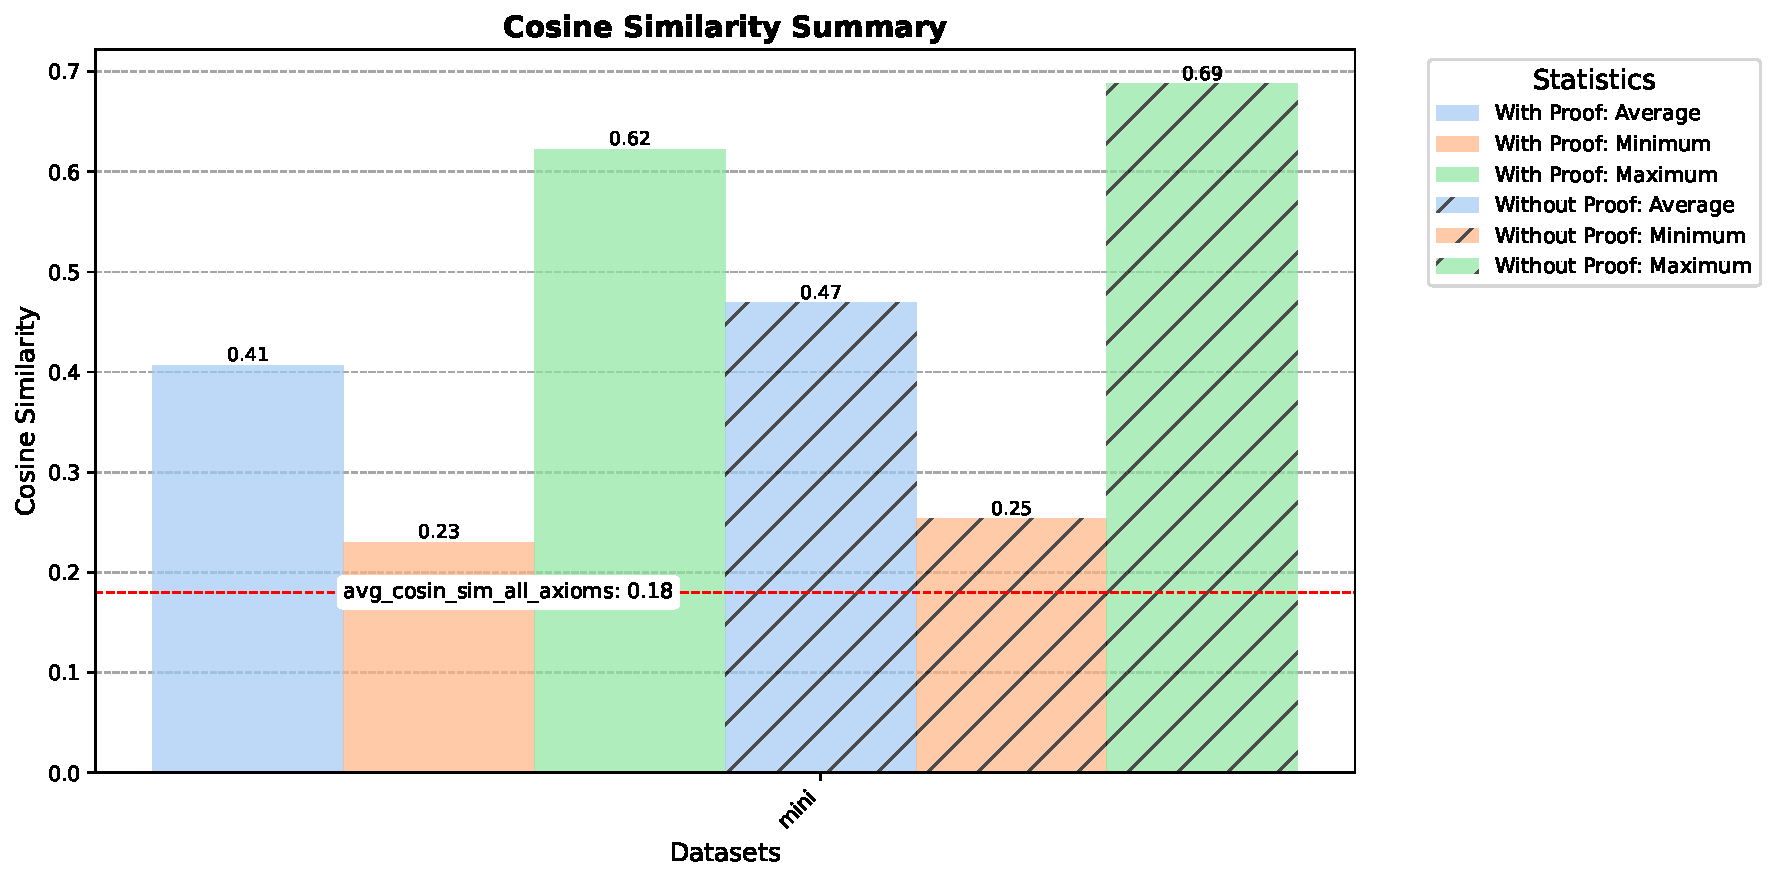
\includegraphics[width=\textwidth]{cosine_similarity_mini_noAdded_summary.pdf}
    \caption{Cosine similarity distribution}
    \label{fig:cosine_similarity}
\end{figure}
\FloatBarrier

The average cosine similarity in cases where a proof was found is 0.41, while it is slightly higher—0.47—when no proof was found. The minimum and maximum similarity values follow a similar trend, with successful proofs ranging from 0.23 to 0.62, and unsuccessful ones from 0.25 to 0.69. The red dashed line represents the average cosine similarity of a conjecture to all axioms in Adimen-SUMO, which is 0.18.

The average cosine similarity between the conjecture and the 160 nearest axioms is slightly lower in cases where a proof was found compared to those where no proof was derived. This suggests that an excessively high cosine similarity may restrict the search space too much, making the selection of axioms overly specific and limiting the prover's ability to construct a valid proof. This indicates that proving a conjecture may require bridging different concepts rather than simply refining closely related axioms.


\section{Expanding Axiom Selection Beyond Semantic and Syntactic Methods}

As previously observed, the pure combination of syntactic and semantic selection methods does not cover a sufficiently broad range of proofs. The results show that conjectures without a successful proof tend to have a higher cosine similarity to their 160 nearest axioms. This suggests that relying solely on semantic and syntactic similarity is not enough. A oberly-specific selection of axioms can lead to missing essential axioms, ultimately preventing the prover from finding a proof.

Since theorem provers, as described in \ref{chapter-introduction}, rely on simplification steps using available axioms, it becomes evident that additional axioms enabling these simplifications are required. Without such axioms, the prover lacks the necessary transformation rules to progress toward a proof.

To identify core axioms, Prover E was executed in auto mode across all 8,010 WhiteBoxTruth tests. In this mode, the prover automatically determines the optimal SInE parameters and applies a search heuristic best suited for each conjecture. After running all tests, the 25 axioms that appeared most frequently in successful proofs were selected as core axioms.

\begin{Pseudocode}[morekeywords = {add, create}, deletekeywords={to}, numbers=left,
    caption = {Prover E configuration}]
    eprover --auto --tstp-format --soft-cpu-limit=15
\end{Pseudocode}


The choice of these axioms is based on their practical relevance in proof construction. Since they are consistently used in successful proofs, they likely provide essential logical connections and simplifications that improve the theorem prover's efficiency.

An example of a core axiom from Adimen-SUMO that facilitates inference is:


\begin{Pseudocode}[morekeywords = {add, create}, deletekeywords={to}, numbers=left, caption = {Example core axiom}]
    fof( mergeA594, axiom,
        (![REL]: 
            (
                (
                    p__d__instance(REL,c__BinaryRelation)
                )
                =>
                (
                    (
                        p__d__instance(REL,c__IrreflexiveRelation)
                    )
                    <=>
                    (
                        (![INST]: 
                            (
                                ~ (
                                    p__d__holds3(REL,INST,INST)
                                )
                            )
                        )
                    )
                )
            )
        )
    ).
\end{Pseudocode}


This axiom defines the irreflexive property of certain binary relations. It states that if a relation REL is classified as a binary relation, then it is an irreflexive relation if and only if there exists no instance INST for which REL holds between INST and itself. In simpler terms, this means that for a relation to be irreflexive, it must never relate an entity to itself.

Such an axiom is fundamental in reasoning about relational structures, as many logical proofs rely on distinguishing between reflexive and irreflexive relations. Without it, the prover may struggle to validate properties of relations that are essential for defining hierarchical and ordering constraints. Including these core axioms in the selection process ensures that theorem proving is not only driven by semantic and syntactic similarity but also by foundational logical principles necessary for accurate inference.

To increase the likelihood of selecting relevant core axioms without significantly expanding their number, a SInE strategy was applied to the 25 core axioms with a benevolence value of 1 and a recursion depth of 1. The axioms selected through this process were then combined with those obtained from the \textit{union}-based selection method, ensuring that both frequently used and structurally relevant axioms were included. Applying this on the same 1.000 WhiteboxTruthTests as before, 286 proofs could be found in the \textit{enhanced-union} run.

\begin{figure}[h!]
    \centering
    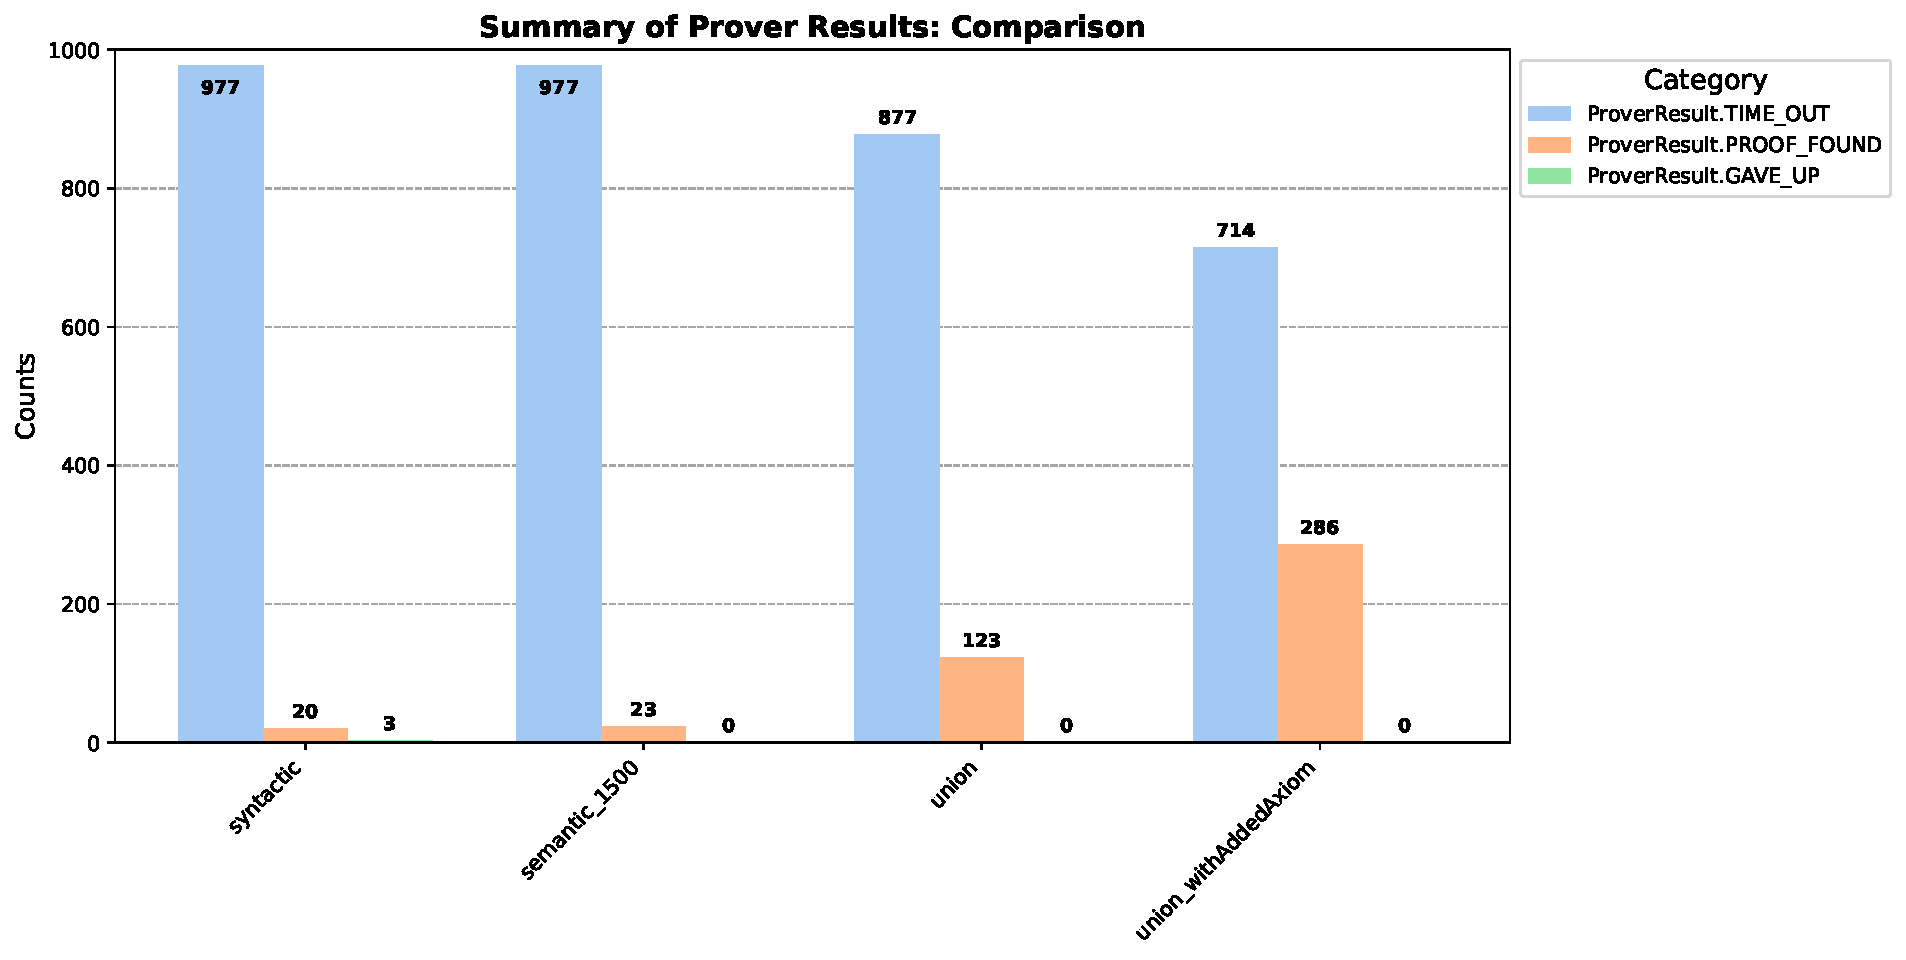
\includegraphics[width=\textwidth]{standard_mode_output.pdf}
    \caption{Summary of prover results with core axioms}
    \label{fig:prover_results_with_core_axioms}
\end{figure}
\FloatBarrier

The \textit{union} run successfully found 123 proofs. After adding the core axioms, the number of proofs increased by 163, resulting in a total of 286 proofs. A closer analysis showed that all 123 proofs from the \textit{union} run were a subset of the proofs found when core axioms were included. 

\begin{equation}
    P_{\text{union}} \subseteq P_{\text{core}} \cup P_{\text{union}}
\end{equation}
where \( P_{\text{union}} \) represents the set of proofs found in the \textit{union} run and \( P_{\text{core}} \) represents the set of proofs found after adding core axioms.


This suggests that adding core axioms plays a crucial role in enabling the prover to find proofs that would otherwise remain undiscovered.


\section{Comparison of Large Language Models}

As previously observed, adding frequently used axioms to the set selected by the \textit{union} process significantly increases the number of proofs that Prover E can find. In the initial setup, a model embedding into 384 dimensions was used. To assess whether the number of dimensions and the size of the model impact proof discovery, the same procedure is repeated using a different model, all-mpnet-base-v2.

The two models differ in several key aspects, including sequence length, embedding dimensions, and overall model size. The following table provides a comparison:

\begin{table}[h]
    \centering
    \begin{tabular}{lcc}
        \hline
        & \textbf{all-mpnet-base-v2} & \textbf{all-MiniLM-L6-v2} \\
        \hline
        Max Sequence Length & 384 & 256 \\
        Embedding Dimensions & 768 & 384 \\
        Model Size & 420MB & 80MB \\
        Training Data & 1B+ training pairs & 1B+ training pairs \\
        \hline
    \end{tabular}
    \caption{Comparison of embedding models used in axiom selection.}
    \label{tab:model_comparison}
\end{table}

The difference of the two models can be seen by the mean sinus similarity of the sample WhiteBoxTruth tests to all axioms in the Adimen-SUMO Ontology.


\begin{table}[h]
    \centering
    \begin{tabular}{lcc}
        \hline
        & \textbf{all-mpnet-base-v2} & \textbf{all-MiniLM-L6-v2} \\
        \hline
        Mean cosine similarity & 0.23 & 0.18 \\
        \hline
    \end{tabular}
    \caption{Mean cosine similarity of test-sample to ontology}
    \label{tab:model_comparison_2}
\end{table}

The all-mpnet-base-v2 model exhibits a significantly higher mean cosine similarity between the sample test conjectures and all axioms in Adimen-SUMO. As previously observed, a high cosine similarity can restrict the search space for the prover, making it necessary to include core axioms to improve proof success. To examine this effect, the prover was run in \textit{union} mode using the all-mpnet-base-v2 model and again in \textit{union} mode with the addition of the previously identified core axioms.

\begin{figure}[h!]
    \centering
    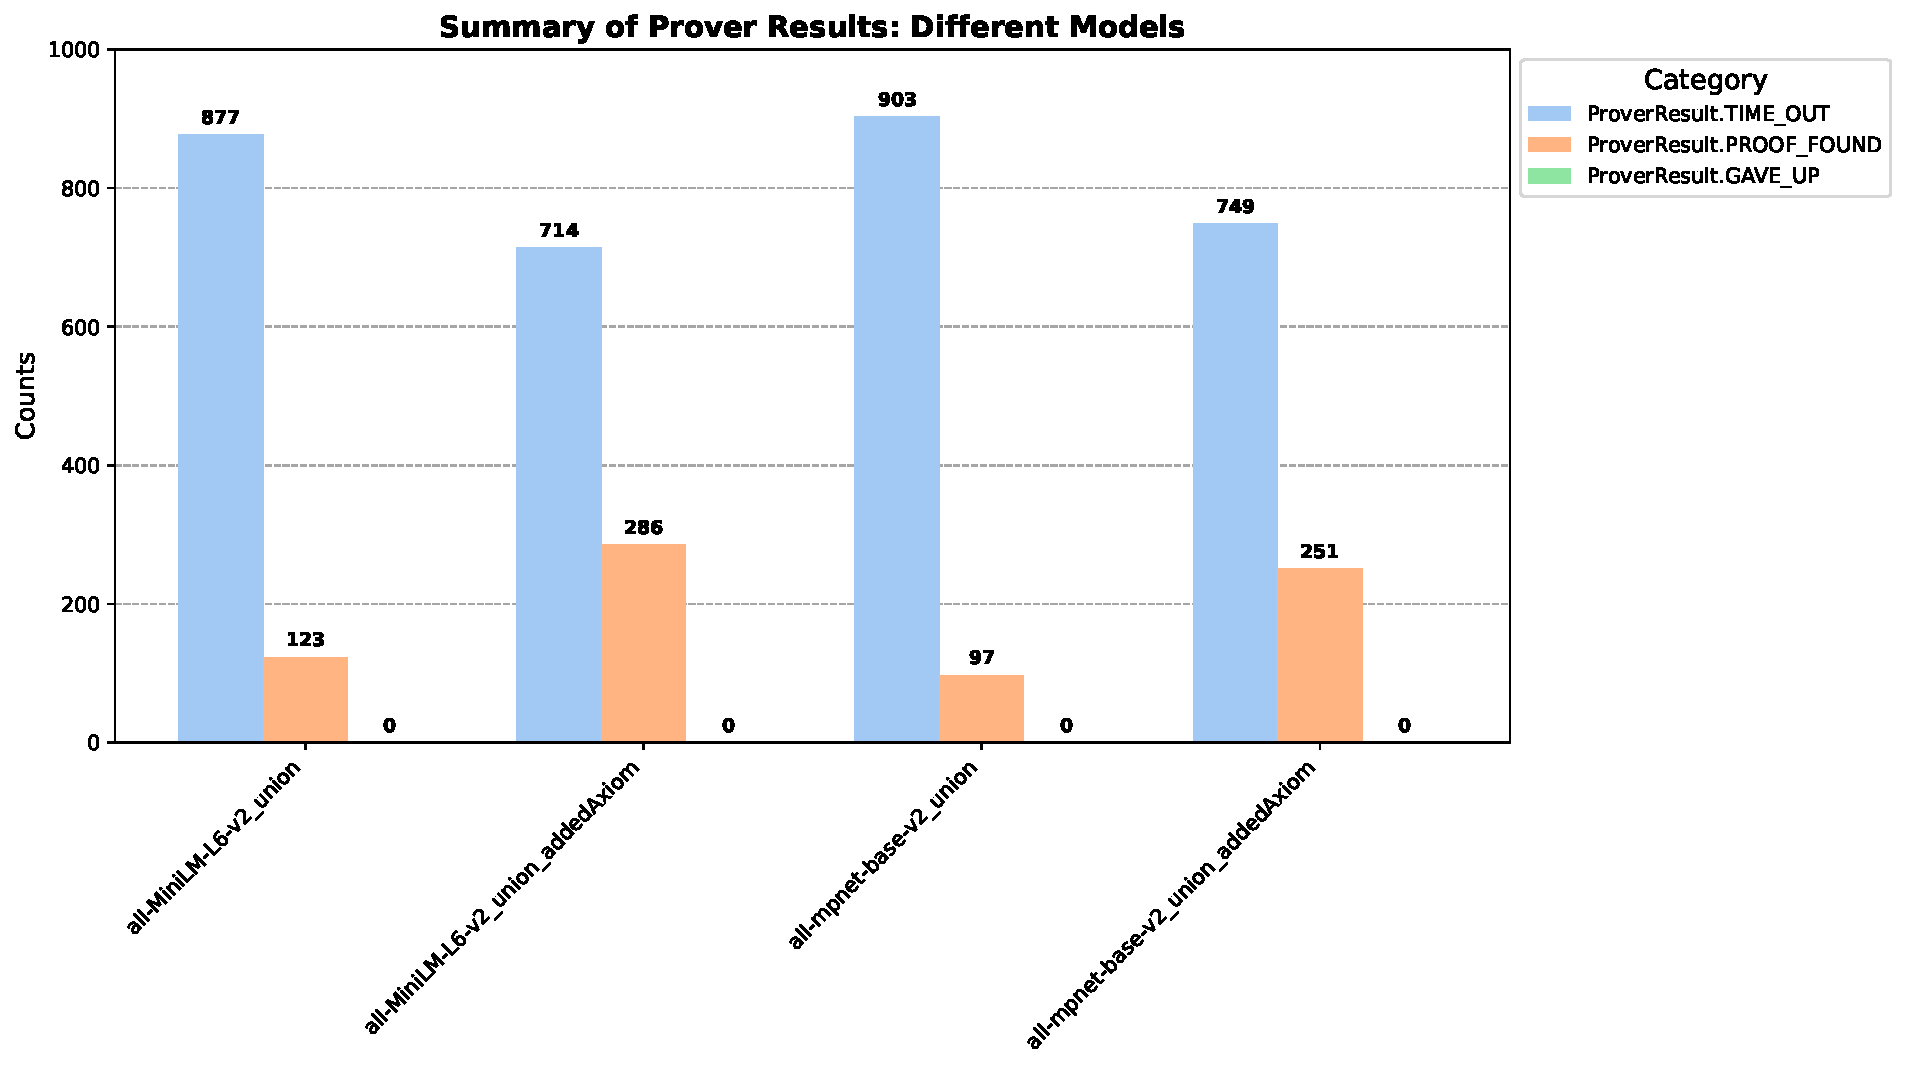
\includegraphics[width=\textwidth]{different_mode_output.pdf}
    \caption{Summary of prover results with different models}
    \label{fig:results_different_models}
\end{figure}        
\FloatBarrier

The increased cosine similarity resulted in fewer proofs being found in \textit{union} mode. The all-mpnet-base-v2 model produced only 97 proofs in the \textit{union} run, compared to 123 proofs found using the smaller model. Similarly, the number of proofs in the \textit{enhanced-union} run was lower than in the corresponding run with the smaller model. Despite this, adding core axioms still led to an increase of 154 additional proofs, reinforcing their importance in theorem proving.

The results suggest that while the larger model provides more accurate embeddings, its higher semantic precision appears to require a broader or more refined selection of axioms to perform as effectively as the smaller model. This indicates that adjustments in axiom selection strategies may be necessary when using higher-dimensional embeddings to ensure optimal prover performance.


\section{Evaluation of Theorem Prover Configurations}

Up to this point, all runs have been conducted using Prover E's standard mode without any specific configurations. To determine whether adding core axioms remains beneficial when the prover operates under specialized settings, two different modes of Prover E will be examined.

Prover E offers specialized modes that automatically adjust search parameters based on the characteristics of the given problem.

\begin{definition}
    \textit{--satauto mode}: Choose literal selection strategy, clause evalua-
    tion heuristic, term ordering and other search
    parameters automagically, based on problem fea-
    tures \cite{schulz2019eprover}.
\end{definition}

\begin{definition}
    \textit{--auto mode}: As --satauto, but add heuristic specification
    pruning using one of several instantiation of the
    SInE algorithm for large specifications.
    This makes the prover potentially incomplete \cite{schulz2019eprover}.
\end{definition}


The impact of different selection strategies on theorem proving performance is evaluated by comparing Prover E's \textit{--satauto} mode under three conditions: running on the full ontology without pre-selection, using \textit{union} mode to pre-slice the search space, and applying \textit{-union} mode. The results are summarized in the following figure:

\begin{figure}[h!]
    \centering
    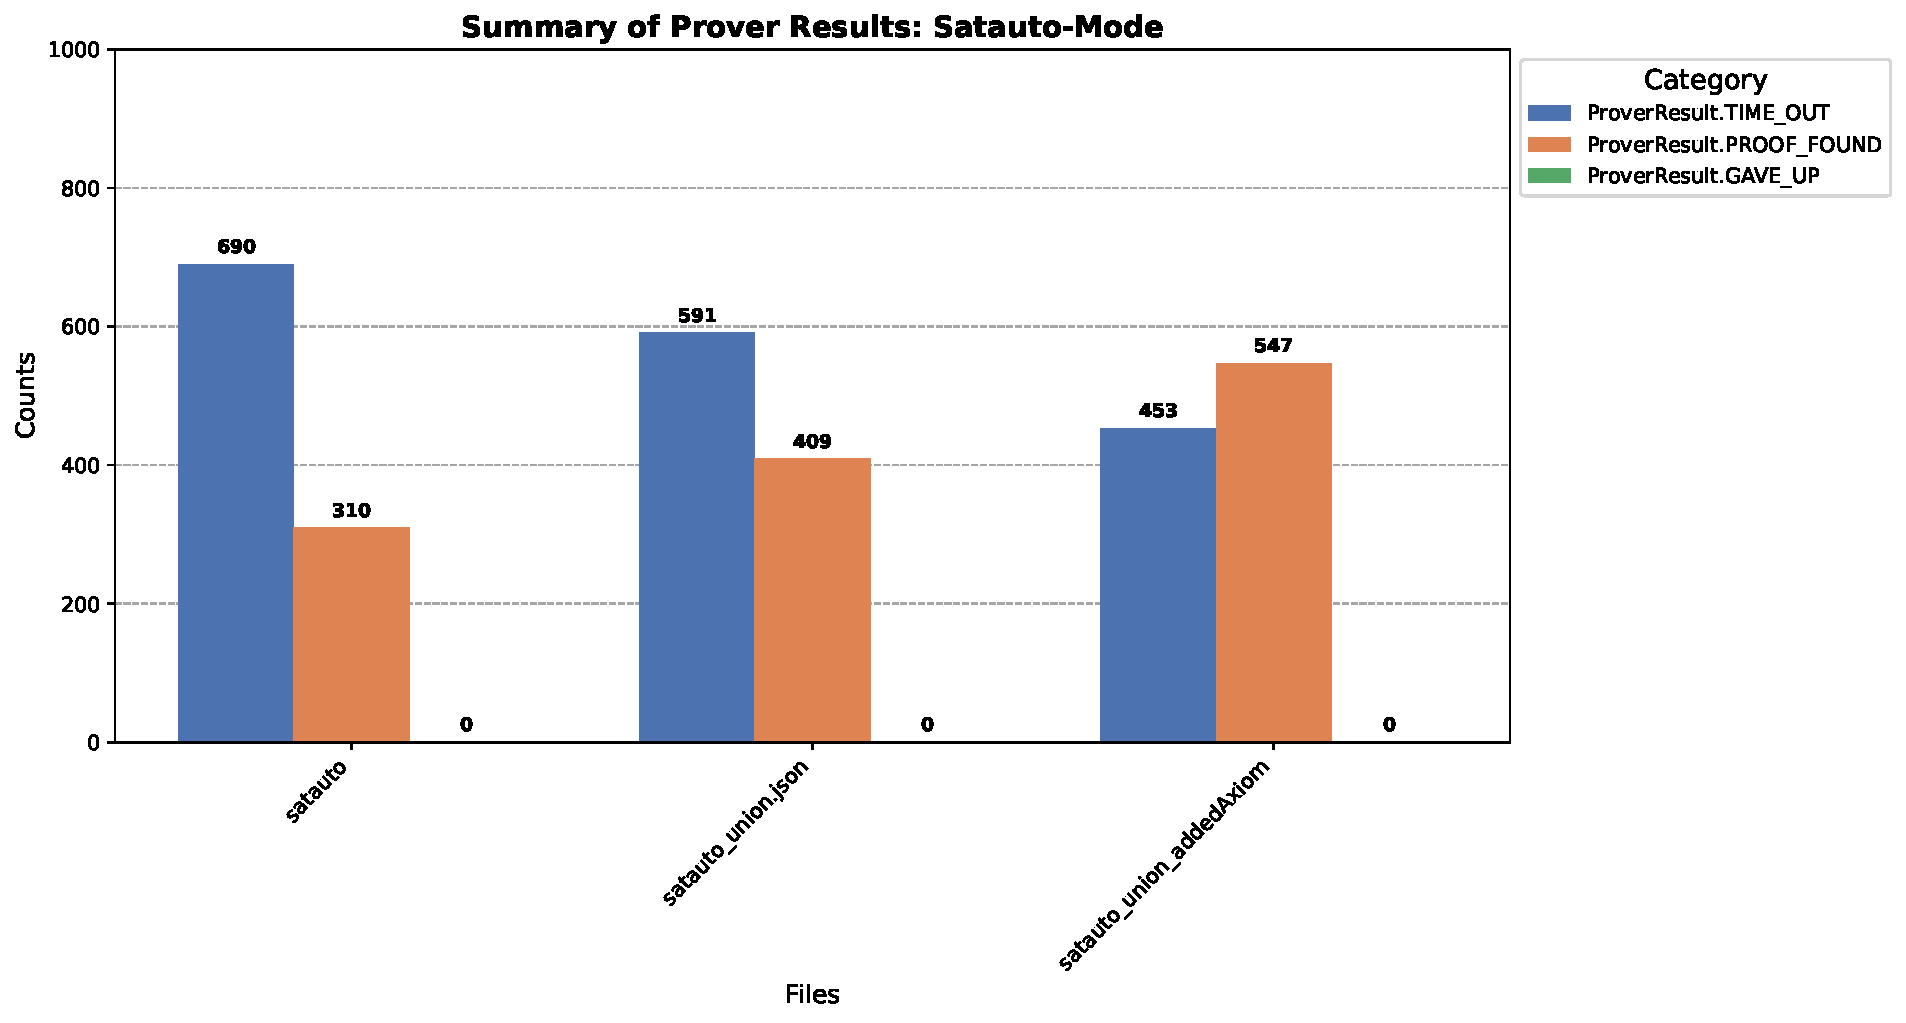
\includegraphics[width=\textwidth]{satauto_mode_output.pdf}
    \caption{Summary of prover results in Satauto mode}
    \label{fig:prover_results_satauto}
\end{figure}
\FloatBarrier

With 310 proofs found, it is evident that automatic selection strategies for literal selection, clause evaluation, and term ordering significantly impact the prover's performance. However, reducing the search space using a combination of syntactic and semantic selection further improves the results. In \textit{enhanced-union} mode, the prover successfully found 509 out of 1,000 proofs, marking the first case where more proofs were found than not.

The same evaluation is then performed in \textit{--auto} mode, where Prover E additionally applies optionally a SInE.

\begin{figure}[h!]
    \centering
    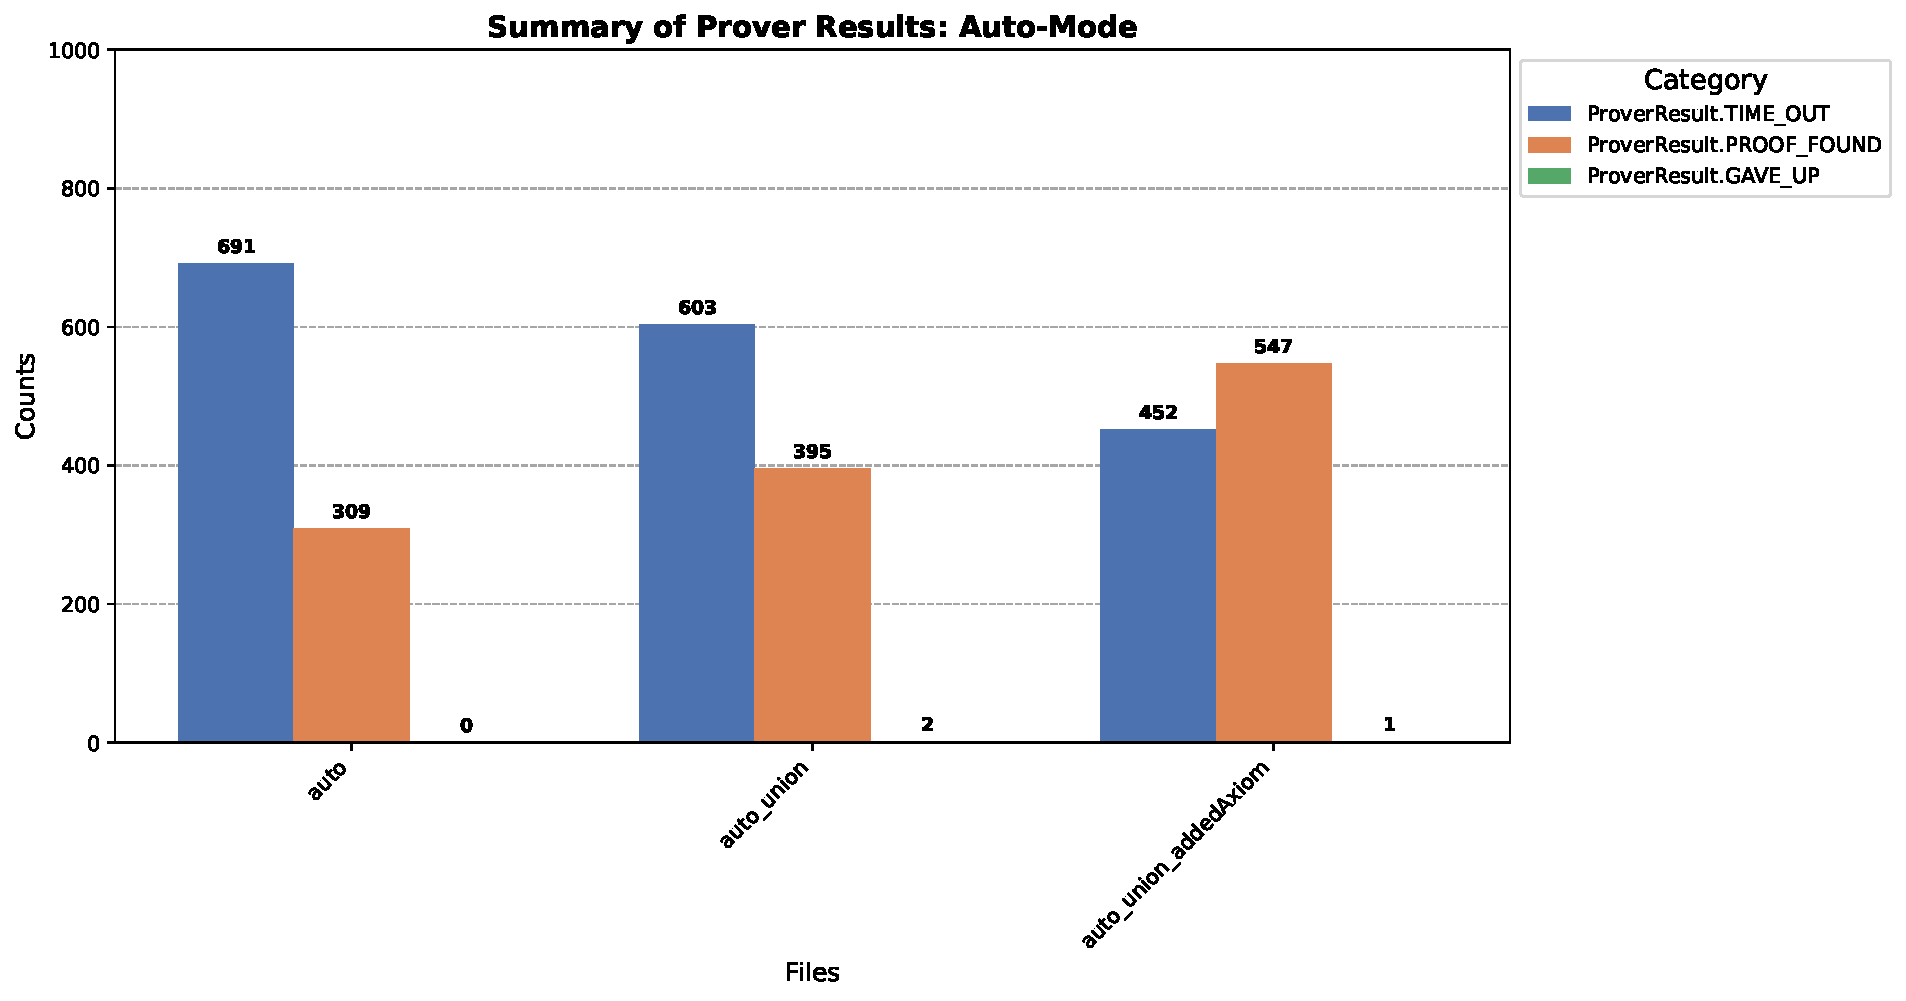
\includegraphics[width=\textwidth]{auto_mode_output.pdf}
    \caption{Summary of prover results in Auto mode}
    \label{fig:prover_results_auto}
\end{figure}
\FloatBarrier

The results are comparable to those in \textit{--satauto} mode. Since the search space was pre-sliced before execution, the additional heuristic slicing in \textit{--auto} mode does not significantly alter performance.

Overall, restricting the search space through a combined syntactic and semantic selection process, supplemented by core axioms, consistently improves the prover’s performance. These results highlight the importance of carefully structuring axiom selection to balance relevance and efficiency in theorem proving.

\section{Impact of Search Space Limitation on Proof Time}

To determine whether restricting the search space influences the time required for Prover E to find a proof, the time taken in different configurations is analyzed. The evaluation compares three scenarios: \textit{standard} mode, \textit{union} mode, and \textit{enhanced-union} mode, while Prover E is in all szenarios run in \textit{--auto} mode.

\begin{figure}[h!]
    \centering
    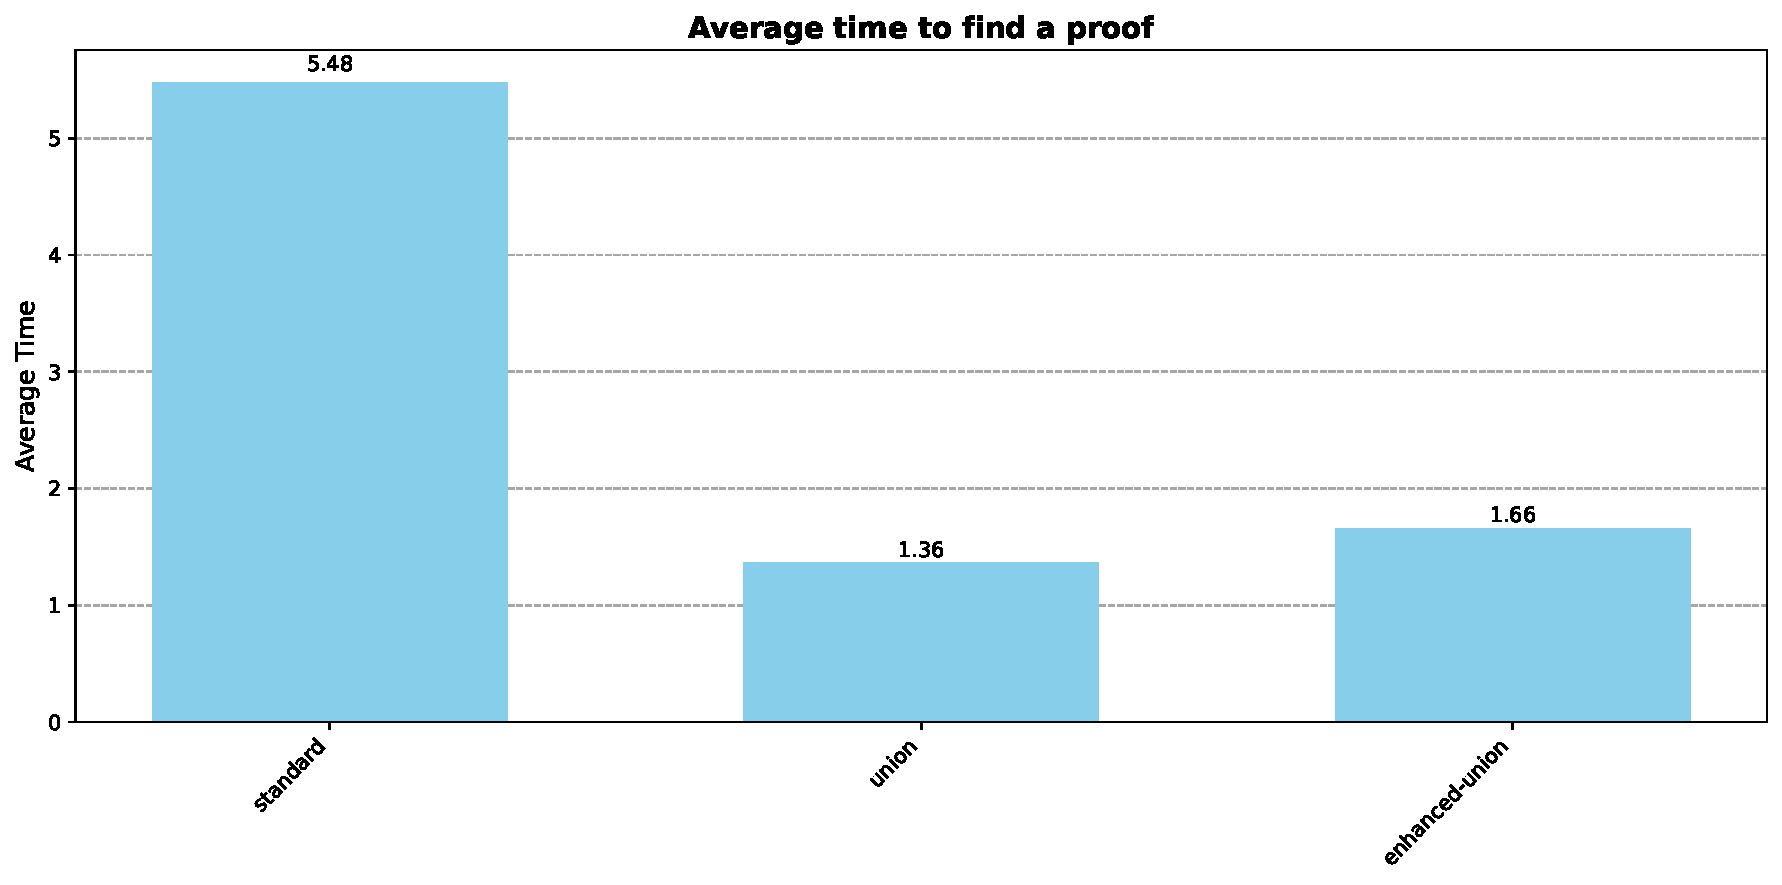
\includegraphics[width=\textwidth]{time_to_find_proof.pdf}
    \caption{Time required for Prover E to find a proof}
    \label{fig:time_different_mode_1}
\end{figure}        
\FloatBarrier

The results show that limiting the search space significantly improves proof discovery speed. In \textit{union} mode, the prover operates more efficiently by focusing on a smaller yet relevant subset of axioms. However, when core axioms are added, the search space expands slightly, leading to a marginal increase in proof time. Despite this, the overall performance remains better than in the \textit{standard} mode, indicating that reducing unnecessary axioms outweighs the added complexity introduced by core axioms.

To further examine the effect of search space limitation, the time required to find proofs common to different configurations is compared. The following figure presents the average time taken by the first method listed to find the same proofs that were already identified by the second.

\begin{figure}[h!]
    \centering
    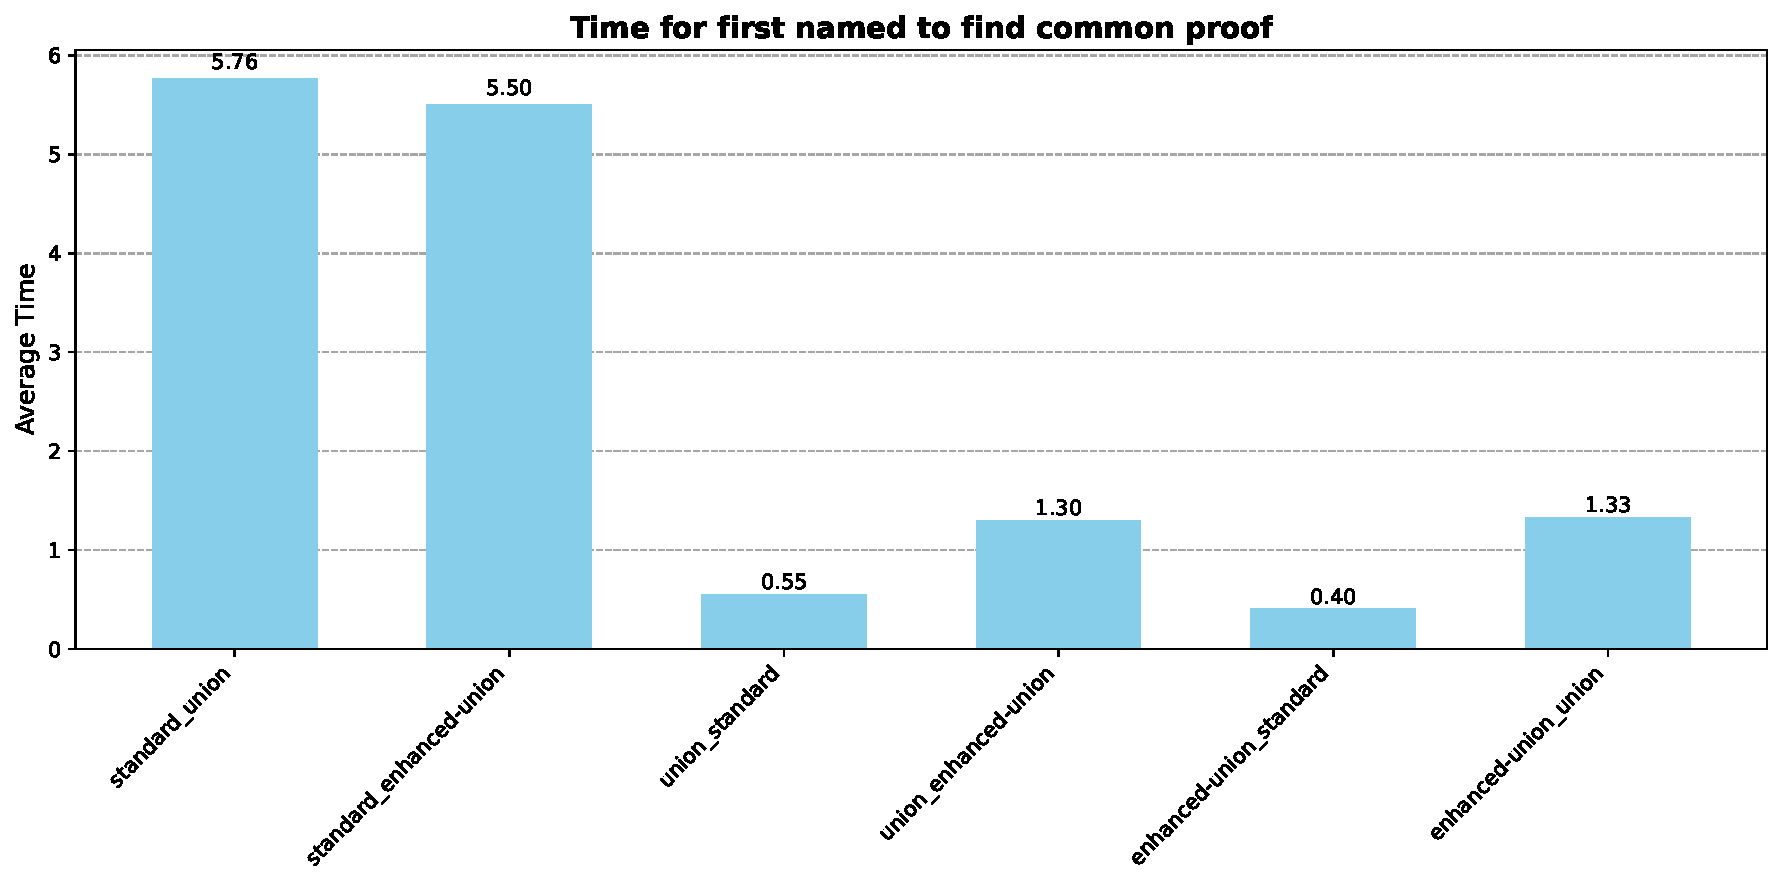
\includegraphics[width=\textwidth]{time_to_find_common_proof.pdf}
    \caption{Average time required to find common proofs}
    \label{fig:time_different_mode}
\end{figure}        
\FloatBarrier

The trend remains consistent—limiting the search space leads to faster proof discovery. When axioms are pre-selected, Prover E spends less time exploring irrelevant information, allowing it to reach conclusions more efficiently. These results further support the importance of a well-structured selection process in optimizing theorem proving performance.


\section{Different prover}
To evaluate whether the proposed adjustments are effective across different theorem provers, the same process is applied using the Vampire prover. By default, Vampire runs in an optimized mode that automatically selects the best configuration, making it comparable to the auto mode in Prover E. As before, the prover is tested in three scenarios: running on the full ontology without pre-selection, using \textit{union} mode, and applying \textit{enhanced-union} mode.

\begin{figure}[h!]
    \centering
    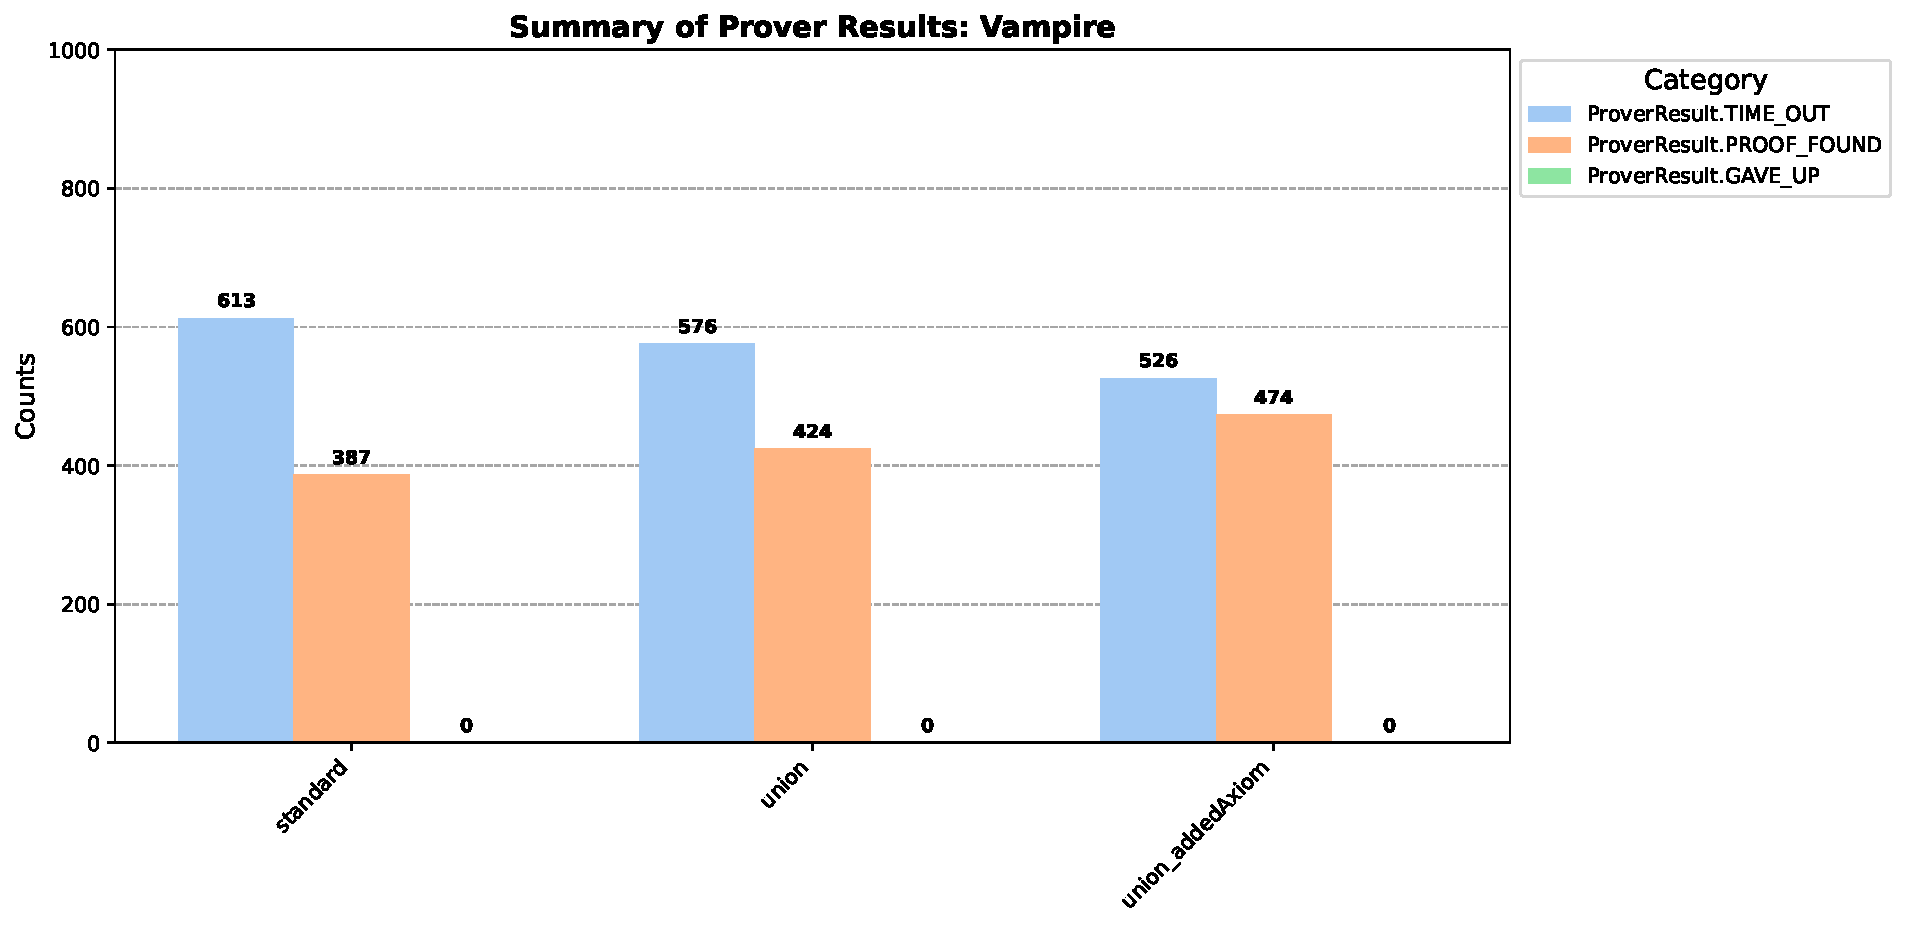
\includegraphics[width=\textwidth]{vampire_mode_output.pdf}
    \caption{Summary of prover Vampire}
    \label{fig:prover_results_vampire}
\end{figure}
\FloatBarrier

Similar to Prover E in \text{--satauto} and \textit{--auto} mode, Vampire successfully finds a large number of proofs in its default configuration. However, the results show the same trend as before—both \textit{union} mode and \textit{enhanced-union} mode further improve performance.
 

% !!!!!!!!!!!!!!!!!!!!!!!!!!!!!!!!!!
% !!! Your action is needed here !!!
% !!!!!!!!!!!!!!!!!!!!!!!!!!!!!!!!!!

\chapter{Conclusion}
\label{chapter-conclusion}
This thesis examined the impact of incorporating frequently used axioms, referred to as core axioms, into the axiom selection process of automated theorem provers. The hypothesis was that adding these axioms, which appear frequently in successful proofs, would improve proof success rates by providing necessary inference steps. To evaluate this, a combination of syntactic and semantic axiom selection strategies was explored, and the results were analyzed across different configurations and theorem provers.

The experiments showed that purely semantic and syntactic selection strategies are insufficient for maximizing proof success. While semantic embeddings allow for meaningful axiom selection, the results indicated that an overly strict focus on similarity can restrict the prover’s search space too much, limiting proof discovery. The syntactic approach, although effective in reducing the search space, also showed limitations when used alone. The integration of both methods in a \textit{union}-based approach improved performance, but adding core axioms led to the most significant increase in proofs found.

The evaluation confirmed that theorem provers benefit from structured axiom selection, especially when core axioms are included. In standard mode, Prover E found 123 proofs using \textit{union}-based selection, while the addition of core axioms increased this number to 286. Similar trends were observed across different prover settings, including \textit{--satauto} and \textit{--auto} mode, as well as in the Vampire prover. In all cases, restricting the search space through a combination of selection strategies enhanced proof success while maintaining efficiency.

Another key finding was the relationship between search space limitation and proof time. The results showed that selecting relevant axioms reduced the time needed to find proofs. However, adding core axioms slightly increased proof time due to the expanded search space, though the overall efficiency gain from improved proof success outweighed this effect.

An additional comparison was conducted using different embedding models to assess whether model size and embedding dimensionality influence theorem proving performance. The all-mpnet-base-v2 (mpnet) model produced embeddings with higher cosine similarity between conjectures and axioms than the all-MiniLM-L6-v2 model (mini). However, the increased similarity resulted in fewer proofs being found, reinforcing the observation that a balance between similarity and search space flexibility is needed. 

The findings demonstrate that effective axiom selection is critical in automated theorem proving. The combination of syntactic filtering, semantic embeddings, and frequently used core axioms provides a well-structured selection process that enhances proof discovery. These results suggest that theorem proving can be further optimized by refining axiom selection methods, balancing search space reduction with the need for inference-enabling axioms.

\chapter{Future work}
\label{chapter-futerwork}

While the current approach demonstrates the effectiveness of combining syntactic and semantic selection with core axioms, several aspects of the configuration could be further optimized. One key area for improvement is analyzing the impact of different parameter settings, such as the number of closest axioms \( k \) and the specific SInE parameters used. Adjusting these values dynamically based on the complexity of the conjecture or the structure of the selected axioms could lead to further performance gains.

Another promising direction is the dynamic selection of core axioms. The current method identifies frequently used axioms across multiple proofs, but this selection remains static. A more adaptive approach could refine core axioms on a per-conjecture basis, ensuring that the most relevant axioms are always included.



% Normally, the bibliography comes next at this point. Do *not* (try
% to) include further indices and tables like an index or
% a list of figures or a list of tables or such things. Nobody
% actually uses them and they just use up space. 
%
% You *can* however include a glossary, if this seems appropriate. It
% goes here as an unnumbered chapter. Most thesis will *not* need a
% glossary: a well-written text (re)explains strange words and
% concepts as necessary. However, there are situations where a
% glossary may be helpful.

%%%
% 
% Bibliographies
%
%%%
%
% The uzl-thesis class will load biblatex for the bibliography
% management. This is a powerful package, see its documentation for
% details. The styles will be setup correctly and automatically by
% choosing one of the two style keys as described earlier.
%
% In order for the bibliography to work, run latex in the following
% order (which is the standard order):
% 
% > lualatex thesis-example
% > bibtex thesis-example
% > lualatex thesis-example
% 
% Add BibTeX files using \addbibresource or use the {bibtex entries}
% environment (see below).
%
%%%
%
% Although everyting is normally setup automatically, you can change
% the options passed to biblatex using the key 'biblatex';
% for instance,
%
%   \UzLThesisSetup{biblatex={firstinits=false}}
%
% will switch off shortened first names. Normally, you will not need
% this key in your preamble. 
% 
% Note that the bibtex program is used as the 'backend' of biblatex
% by default (rather than biber, which is the preferred program of
% biblatex). This means that you can (and must) run *bibtex* after you
% have run lualatex on your thesis. If you wish to use biber instead
% of bibtex, say 'biblatex={backend=biber}'. 
% 
%%%
%
% The following environment is optional. It allows you to keep the
% bibtex entries for your thesis right here in the thesis file. What
% happens is that each time this tex file is processed, the contents
% of the following environment gets written to the file
% \jobname-bibtex-entries.bib (this file gets overwritten each
% time). Independently, \addbibresource{\jobname-bibtex-entries.bib}
% is always called if the file \jobname-bibtex-entries.bib
% exists. 
%
% In result, you can edit and keep the bibliography's bibtex entries
% right here. If you change something here, run latex, then bibtex,
% then latex once more.
%
% If you would like to manage the bibtex entries in a separate file,
% remove the below environment, delete the \jobname-bibtex-entries.bib
% file and instead write
%
% \addbibresource{filename-of-your-bibtex-file.bib}
%
% in the preamble.
%
%%%


\end{document}
